\documentclass[11pt]{article}

    \usepackage[breakable]{tcolorbox}
    \usepackage{parskip} % Stop auto-indenting (to mimic markdown behaviour)
    

    % Basic figure setup, for now with no caption control since it's done
    % automatically by Pandoc (which extracts ![](path) syntax from Markdown).
    \usepackage{graphicx}
    % Keep aspect ratio if custom image width or height is specified
    \setkeys{Gin}{keepaspectratio}
    % Maintain compatibility with old templates. Remove in nbconvert 6.0
    \let\Oldincludegraphics\includegraphics
    % Ensure that by default, figures have no caption (until we provide a
    % proper Figure object with a Caption API and a way to capture that
    % in the conversion process - todo).
    \usepackage{caption}
    \DeclareCaptionFormat{nocaption}{}
    \captionsetup{format=nocaption,aboveskip=0pt,belowskip=0pt}

    \usepackage{float}
    \floatplacement{figure}{H} % forces figures to be placed at the correct location
    \usepackage{xcolor} % Allow colors to be defined
    \usepackage{enumerate} % Needed for markdown enumerations to work
    \usepackage{geometry} % Used to adjust the document margins
    \usepackage{amsmath} % Equations
    \usepackage{amssymb} % Equations
    \usepackage{textcomp} % defines textquotesingle
    % Hack from http://tex.stackexchange.com/a/47451/13684:
    \AtBeginDocument{%
        \def\PYZsq{\textquotesingle}% Upright quotes in Pygmentized code
    }
    \usepackage{upquote} % Upright quotes for verbatim code
    \usepackage{eurosym} % defines \euro
	\usepackage{cancel}
    \usepackage{iftex}
    \ifPDFTeX
        \usepackage[T1]{fontenc}
        \IfFileExists{alphabeta.sty}{
              \usepackage{alphabeta}
          }{
              \usepackage[mathletters]{ucs}
              \usepackage[utf8x]{inputenc}
          }
    \else
        \usepackage{fontspec}
        \usepackage{unicode-math}
    \fi

    \usepackage{fancyvrb} % verbatim replacement that allows latex
    \usepackage{grffile} % extends the file name processing of package graphics
                         % to support a larger range
    \makeatletter % fix for old versions of grffile with XeLaTeX
    \@ifpackagelater{grffile}{2019/11/01}
    {
      % Do nothing on new versions
    }
    {
      \def\Gread@@xetex#1{%
        \IfFileExists{"\Gin@base".bb}%
        {\Gread@eps{\Gin@base.bb}}%
        {\Gread@@xetex@aux#1}%
      }
    }
    \makeatother
    \usepackage[Export]{adjustbox} % Used to constrain images to a maximum size
    \adjustboxset{max size={0.9\linewidth}{0.9\paperheight}}

    % The hyperref package gives us a pdf with properly built
    % internal navigation ('pdf bookmarks' for the table of contents,
    % internal cross-reference links, web links for URLs, etc.)
    \usepackage{hyperref}
    % The default LaTeX title has an obnoxious amount of whitespace. By default,
    % titling removes some of it. It also provides customization options.
    \usepackage{titling}
    \usepackage{longtable} % longtable support required by pandoc >1.10
    \usepackage{booktabs}  % table support for pandoc > 1.12.2
    \usepackage{array}     % table support for pandoc >= 2.11.3
    \usepackage{calc}      % table minipage width calculation for pandoc >= 2.11.1
    \usepackage[inline]{enumitem} % IRkernel/repr support (it uses the enumerate* environment)
    \usepackage[normalem]{ulem} % ulem is needed to support strikethroughs (\sout)
                                % normalem makes italics be italics, not underlines
    \usepackage{soul}      % strikethrough (\st) support for pandoc >= 3.0.0
    \usepackage{mathrsfs}

    

    
    % Colors for the hyperref package
    \definecolor{urlcolor}{rgb}{0,.145,.698}
    \definecolor{linkcolor}{rgb}{.71,0.21,0.01}
    \definecolor{citecolor}{rgb}{.12,.54,.11}

    % ANSI colors
    \definecolor{ansi-black}{HTML}{3E424D}
    \definecolor{ansi-black-intense}{HTML}{282C36}
    \definecolor{ansi-red}{HTML}{E75C58}
    \definecolor{ansi-red-intense}{HTML}{B22B31}
    \definecolor{ansi-green}{HTML}{00A250}
    \definecolor{ansi-green-intense}{HTML}{007427}
    \definecolor{ansi-yellow}{HTML}{DDB62B}
    \definecolor{ansi-yellow-intense}{HTML}{B27D12}
    \definecolor{ansi-blue}{HTML}{208FFB}
    \definecolor{ansi-blue-intense}{HTML}{0065CA}
    \definecolor{ansi-magenta}{HTML}{D160C4}
    \definecolor{ansi-magenta-intense}{HTML}{A03196}
    \definecolor{ansi-cyan}{HTML}{60C6C8}
    \definecolor{ansi-cyan-intense}{HTML}{258F8F}
    \definecolor{ansi-white}{HTML}{C5C1B4}
    \definecolor{ansi-white-intense}{HTML}{A1A6B2}
    \definecolor{ansi-default-inverse-fg}{HTML}{FFFFFF}
    \definecolor{ansi-default-inverse-bg}{HTML}{000000}

    % common color for the border for error outputs.
    \definecolor{outerrorbackground}{HTML}{FFDFDF}

    % commands and environments needed by pandoc snippets
    % extracted from the output of `pandoc -s`
    \providecommand{\tightlist}{%
      \setlength{\itemsep}{0pt}\setlength{\parskip}{0pt}}
    \DefineVerbatimEnvironment{Highlighting}{Verbatim}{commandchars=\\\{\}}
    % Add ',fontsize=\small' for more characters per line
    \newenvironment{Shaded}{}{}
    \newcommand{\KeywordTok}[1]{\textcolor[rgb]{0.00,0.44,0.13}{\textbf{{#1}}}}
    \newcommand{\DataTypeTok}[1]{\textcolor[rgb]{0.56,0.13,0.00}{{#1}}}
    \newcommand{\DecValTok}[1]{\textcolor[rgb]{0.25,0.63,0.44}{{#1}}}
    \newcommand{\BaseNTok}[1]{\textcolor[rgb]{0.25,0.63,0.44}{{#1}}}
    \newcommand{\FloatTok}[1]{\textcolor[rgb]{0.25,0.63,0.44}{{#1}}}
    \newcommand{\CharTok}[1]{\textcolor[rgb]{0.25,0.44,0.63}{{#1}}}
    \newcommand{\StringTok}[1]{\textcolor[rgb]{0.25,0.44,0.63}{{#1}}}
    \newcommand{\CommentTok}[1]{\textcolor[rgb]{0.38,0.63,0.69}{\textit{{#1}}}}
    \newcommand{\OtherTok}[1]{\textcolor[rgb]{0.00,0.44,0.13}{{#1}}}
    \newcommand{\AlertTok}[1]{\textcolor[rgb]{1.00,0.00,0.00}{\textbf{{#1}}}}
    \newcommand{\FunctionTok}[1]{\textcolor[rgb]{0.02,0.16,0.49}{{#1}}}
    \newcommand{\RegionMarkerTok}[1]{{#1}}
    \newcommand{\ErrorTok}[1]{\textcolor[rgb]{1.00,0.00,0.00}{\textbf{{#1}}}}
    \newcommand{\NormalTok}[1]{{#1}}

    % Additional commands for more recent versions of Pandoc
    \newcommand{\ConstantTok}[1]{\textcolor[rgb]{0.53,0.00,0.00}{{#1}}}
    \newcommand{\SpecialCharTok}[1]{\textcolor[rgb]{0.25,0.44,0.63}{{#1}}}
    \newcommand{\VerbatimStringTok}[1]{\textcolor[rgb]{0.25,0.44,0.63}{{#1}}}
    \newcommand{\SpecialStringTok}[1]{\textcolor[rgb]{0.73,0.40,0.53}{{#1}}}
    \newcommand{\ImportTok}[1]{{#1}}
    \newcommand{\DocumentationTok}[1]{\textcolor[rgb]{0.73,0.13,0.13}{\textit{{#1}}}}
    \newcommand{\AnnotationTok}[1]{\textcolor[rgb]{0.38,0.63,0.69}{\textbf{\textit{{#1}}}}}
    \newcommand{\CommentVarTok}[1]{\textcolor[rgb]{0.38,0.63,0.69}{\textbf{\textit{{#1}}}}}
    \newcommand{\VariableTok}[1]{\textcolor[rgb]{0.10,0.09,0.49}{{#1}}}
    \newcommand{\ControlFlowTok}[1]{\textcolor[rgb]{0.00,0.44,0.13}{\textbf{{#1}}}}
    \newcommand{\OperatorTok}[1]{\textcolor[rgb]{0.40,0.40,0.40}{{#1}}}
    \newcommand{\BuiltInTok}[1]{{#1}}
    \newcommand{\ExtensionTok}[1]{{#1}}
    \newcommand{\PreprocessorTok}[1]{\textcolor[rgb]{0.74,0.48,0.00}{{#1}}}
    \newcommand{\AttributeTok}[1]{\textcolor[rgb]{0.49,0.56,0.16}{{#1}}}
    \newcommand{\InformationTok}[1]{\textcolor[rgb]{0.38,0.63,0.69}{\textbf{\textit{{#1}}}}}
    \newcommand{\WarningTok}[1]{\textcolor[rgb]{0.38,0.63,0.69}{\textbf{\textit{{#1}}}}}
    \makeatletter
    \newsavebox\pandoc@box
    \newcommand*\pandocbounded[1]{%
      \sbox\pandoc@box{#1}%
      % scaling factors for width and height
      \Gscale@div\@tempa\textheight{\dimexpr\ht\pandoc@box+\dp\pandoc@box\relax}%
      \Gscale@div\@tempb\linewidth{\wd\pandoc@box}%
      % select the smaller of both
      \ifdim\@tempb\p@<\@tempa\p@
        \let\@tempa\@tempb
      \fi
      % scaling accordingly (\@tempa < 1)
      \ifdim\@tempa\p@<\p@
        \scalebox{\@tempa}{\usebox\pandoc@box}%
      % scaling not needed, use as it is
      \else
        \usebox{\pandoc@box}%
      \fi
    }
    \makeatother

    % Define a nice break command that doesn't care if a line doesn't already
    % exist.
    \def\br{\hspace*{\fill} \\* }
    % Math Jax compatibility definitions
    \def\gt{>}
    \def\lt{<}
    \let\Oldtex\TeX
    \let\Oldlatex\LaTeX
    \renewcommand{\TeX}{\textrm{\Oldtex}}
    \renewcommand{\LaTeX}{\textrm{\Oldlatex}}
    % Document parameters
    % Document title
\title{Report - Part 3 \\ \bigskip  \normalsize Seismic Analysis of High Voltage Power Line Truss}
\date{June 23, 2025}
    
    
% Pygments definitions
\makeatletter
\def\PY@reset{\let\PY@it=\relax \let\PY@bf=\relax%
    \let\PY@ul=\relax \let\PY@tc=\relax%
    \let\PY@bc=\relax \let\PY@ff=\relax}
\def\PY@tok#1{\csname PY@tok@#1\endcsname}
\def\PY@toks#1+{\ifx\relax#1\empty\else%
    \PY@tok{#1}\expandafter\PY@toks\fi}
\def\PY@do#1{\PY@bc{\PY@tc{\PY@ul{%
    \PY@it{\PY@bf{\PY@ff{#1}}}}}}}
\def\PY#1#2{\PY@reset\PY@toks#1+\relax+\PY@do{#2}}

\@namedef{PY@tok@w}{\def\PY@tc##1{\textcolor[rgb]{0.73,0.73,0.73}{##1}}}
\@namedef{PY@tok@c}{\let\PY@it=\textit\def\PY@tc##1{\textcolor[rgb]{0.24,0.48,0.48}{##1}}}
\@namedef{PY@tok@cp}{\def\PY@tc##1{\textcolor[rgb]{0.61,0.40,0.00}{##1}}}
\@namedef{PY@tok@k}{\let\PY@bf=\textbf\def\PY@tc##1{\textcolor[rgb]{0.00,0.50,0.00}{##1}}}
\@namedef{PY@tok@kp}{\def\PY@tc##1{\textcolor[rgb]{0.00,0.50,0.00}{##1}}}
\@namedef{PY@tok@kt}{\def\PY@tc##1{\textcolor[rgb]{0.69,0.00,0.25}{##1}}}
\@namedef{PY@tok@o}{\def\PY@tc##1{\textcolor[rgb]{0.40,0.40,0.40}{##1}}}
\@namedef{PY@tok@ow}{\let\PY@bf=\textbf\def\PY@tc##1{\textcolor[rgb]{0.67,0.13,1.00}{##1}}}
\@namedef{PY@tok@nb}{\def\PY@tc##1{\textcolor[rgb]{0.00,0.50,0.00}{##1}}}
\@namedef{PY@tok@nf}{\def\PY@tc##1{\textcolor[rgb]{0.00,0.00,1.00}{##1}}}
\@namedef{PY@tok@nc}{\let\PY@bf=\textbf\def\PY@tc##1{\textcolor[rgb]{0.00,0.00,1.00}{##1}}}
\@namedef{PY@tok@nn}{\let\PY@bf=\textbf\def\PY@tc##1{\textcolor[rgb]{0.00,0.00,1.00}{##1}}}
\@namedef{PY@tok@ne}{\let\PY@bf=\textbf\def\PY@tc##1{\textcolor[rgb]{0.80,0.25,0.22}{##1}}}
\@namedef{PY@tok@nv}{\def\PY@tc##1{\textcolor[rgb]{0.10,0.09,0.49}{##1}}}
\@namedef{PY@tok@no}{\def\PY@tc##1{\textcolor[rgb]{0.53,0.00,0.00}{##1}}}
\@namedef{PY@tok@nl}{\def\PY@tc##1{\textcolor[rgb]{0.46,0.46,0.00}{##1}}}
\@namedef{PY@tok@ni}{\let\PY@bf=\textbf\def\PY@tc##1{\textcolor[rgb]{0.44,0.44,0.44}{##1}}}
\@namedef{PY@tok@na}{\def\PY@tc##1{\textcolor[rgb]{0.41,0.47,0.13}{##1}}}
\@namedef{PY@tok@nt}{\let\PY@bf=\textbf\def\PY@tc##1{\textcolor[rgb]{0.00,0.50,0.00}{##1}}}
\@namedef{PY@tok@nd}{\def\PY@tc##1{\textcolor[rgb]{0.67,0.13,1.00}{##1}}}
\@namedef{PY@tok@s}{\def\PY@tc##1{\textcolor[rgb]{0.73,0.13,0.13}{##1}}}
\@namedef{PY@tok@sd}{\let\PY@it=\textit\def\PY@tc##1{\textcolor[rgb]{0.73,0.13,0.13}{##1}}}
\@namedef{PY@tok@si}{\let\PY@bf=\textbf\def\PY@tc##1{\textcolor[rgb]{0.64,0.35,0.47}{##1}}}
\@namedef{PY@tok@se}{\let\PY@bf=\textbf\def\PY@tc##1{\textcolor[rgb]{0.67,0.36,0.12}{##1}}}
\@namedef{PY@tok@sr}{\def\PY@tc##1{\textcolor[rgb]{0.64,0.35,0.47}{##1}}}
\@namedef{PY@tok@ss}{\def\PY@tc##1{\textcolor[rgb]{0.10,0.09,0.49}{##1}}}
\@namedef{PY@tok@sx}{\def\PY@tc##1{\textcolor[rgb]{0.00,0.50,0.00}{##1}}}
\@namedef{PY@tok@m}{\def\PY@tc##1{\textcolor[rgb]{0.40,0.40,0.40}{##1}}}
\@namedef{PY@tok@gh}{\let\PY@bf=\textbf\def\PY@tc##1{\textcolor[rgb]{0.00,0.00,0.50}{##1}}}
\@namedef{PY@tok@gu}{\let\PY@bf=\textbf\def\PY@tc##1{\textcolor[rgb]{0.50,0.00,0.50}{##1}}}
\@namedef{PY@tok@gd}{\def\PY@tc##1{\textcolor[rgb]{0.63,0.00,0.00}{##1}}}
\@namedef{PY@tok@gi}{\def\PY@tc##1{\textcolor[rgb]{0.00,0.52,0.00}{##1}}}
\@namedef{PY@tok@gr}{\def\PY@tc##1{\textcolor[rgb]{0.89,0.00,0.00}{##1}}}
\@namedef{PY@tok@ge}{\let\PY@it=\textit}
\@namedef{PY@tok@gs}{\let\PY@bf=\textbf}
\@namedef{PY@tok@ges}{\let\PY@bf=\textbf\let\PY@it=\textit}
\@namedef{PY@tok@gp}{\let\PY@bf=\textbf\def\PY@tc##1{\textcolor[rgb]{0.00,0.00,0.50}{##1}}}
\@namedef{PY@tok@go}{\def\PY@tc##1{\textcolor[rgb]{0.44,0.44,0.44}{##1}}}
\@namedef{PY@tok@gt}{\def\PY@tc##1{\textcolor[rgb]{0.00,0.27,0.87}{##1}}}
\@namedef{PY@tok@err}{\def\PY@bc##1{{\setlength{\fboxsep}{\string -\fboxrule}\fcolorbox[rgb]{1.00,0.00,0.00}{1,1,1}{\strut ##1}}}}
\@namedef{PY@tok@kc}{\let\PY@bf=\textbf\def\PY@tc##1{\textcolor[rgb]{0.00,0.50,0.00}{##1}}}
\@namedef{PY@tok@kd}{\let\PY@bf=\textbf\def\PY@tc##1{\textcolor[rgb]{0.00,0.50,0.00}{##1}}}
\@namedef{PY@tok@kn}{\let\PY@bf=\textbf\def\PY@tc##1{\textcolor[rgb]{0.00,0.50,0.00}{##1}}}
\@namedef{PY@tok@kr}{\let\PY@bf=\textbf\def\PY@tc##1{\textcolor[rgb]{0.00,0.50,0.00}{##1}}}
\@namedef{PY@tok@bp}{\def\PY@tc##1{\textcolor[rgb]{0.00,0.50,0.00}{##1}}}
\@namedef{PY@tok@fm}{\def\PY@tc##1{\textcolor[rgb]{0.00,0.00,1.00}{##1}}}
\@namedef{PY@tok@vc}{\def\PY@tc##1{\textcolor[rgb]{0.10,0.09,0.49}{##1}}}
\@namedef{PY@tok@vg}{\def\PY@tc##1{\textcolor[rgb]{0.10,0.09,0.49}{##1}}}
\@namedef{PY@tok@vi}{\def\PY@tc##1{\textcolor[rgb]{0.10,0.09,0.49}{##1}}}
\@namedef{PY@tok@vm}{\def\PY@tc##1{\textcolor[rgb]{0.10,0.09,0.49}{##1}}}
\@namedef{PY@tok@sa}{\def\PY@tc##1{\textcolor[rgb]{0.73,0.13,0.13}{##1}}}
\@namedef{PY@tok@sb}{\def\PY@tc##1{\textcolor[rgb]{0.73,0.13,0.13}{##1}}}
\@namedef{PY@tok@sc}{\def\PY@tc##1{\textcolor[rgb]{0.73,0.13,0.13}{##1}}}
\@namedef{PY@tok@dl}{\def\PY@tc##1{\textcolor[rgb]{0.73,0.13,0.13}{##1}}}
\@namedef{PY@tok@s2}{\def\PY@tc##1{\textcolor[rgb]{0.73,0.13,0.13}{##1}}}
\@namedef{PY@tok@sh}{\def\PY@tc##1{\textcolor[rgb]{0.73,0.13,0.13}{##1}}}
\@namedef{PY@tok@s1}{\def\PY@tc##1{\textcolor[rgb]{0.73,0.13,0.13}{##1}}}
\@namedef{PY@tok@mb}{\def\PY@tc##1{\textcolor[rgb]{0.40,0.40,0.40}{##1}}}
\@namedef{PY@tok@mf}{\def\PY@tc##1{\textcolor[rgb]{0.40,0.40,0.40}{##1}}}
\@namedef{PY@tok@mh}{\def\PY@tc##1{\textcolor[rgb]{0.40,0.40,0.40}{##1}}}
\@namedef{PY@tok@mi}{\def\PY@tc##1{\textcolor[rgb]{0.40,0.40,0.40}{##1}}}
\@namedef{PY@tok@il}{\def\PY@tc##1{\textcolor[rgb]{0.40,0.40,0.40}{##1}}}
\@namedef{PY@tok@mo}{\def\PY@tc##1{\textcolor[rgb]{0.40,0.40,0.40}{##1}}}
\@namedef{PY@tok@ch}{\let\PY@it=\textit\def\PY@tc##1{\textcolor[rgb]{0.24,0.48,0.48}{##1}}}
\@namedef{PY@tok@cm}{\let\PY@it=\textit\def\PY@tc##1{\textcolor[rgb]{0.24,0.48,0.48}{##1}}}
\@namedef{PY@tok@cpf}{\let\PY@it=\textit\def\PY@tc##1{\textcolor[rgb]{0.24,0.48,0.48}{##1}}}
\@namedef{PY@tok@c1}{\let\PY@it=\textit\def\PY@tc##1{\textcolor[rgb]{0.24,0.48,0.48}{##1}}}
\@namedef{PY@tok@cs}{\let\PY@it=\textit\def\PY@tc##1{\textcolor[rgb]{0.24,0.48,0.48}{##1}}}

\def\PYZbs{\char`\\}
\def\PYZus{\char`\_}
\def\PYZob{\char`\{}
\def\PYZcb{\char`\}}
\def\PYZca{\char`\^}
\def\PYZam{\char`\&}
\def\PYZlt{\char`\<}
\def\PYZgt{\char`\>}
\def\PYZsh{\char`\#}
\def\PYZpc{\char`\%}
\def\PYZdl{\char`\$}
\def\PYZhy{\char`\-}
\def\PYZsq{\char`\'}
\def\PYZdq{\char`\"}
\def\PYZti{\char`\~}
% for compatibility with earlier versions
\def\PYZat{@}
\def\PYZlb{[}
\def\PYZrb{]}
\makeatother


    % For linebreaks inside Verbatim environment from package fancyvrb.
    \makeatletter
        \newbox\Wrappedcontinuationbox
        \newbox\Wrappedvisiblespacebox
        \newcommand*\Wrappedvisiblespace {\textcolor{red}{\textvisiblespace}}
        \newcommand*\Wrappedcontinuationsymbol {\textcolor{red}{\llap{\tiny$\m@th\hookrightarrow$}}}
        \newcommand*\Wrappedcontinuationindent {3ex }
        \newcommand*\Wrappedafterbreak {\kern\Wrappedcontinuationindent\copy\Wrappedcontinuationbox}
        % Take advantage of the already applied Pygments mark-up to insert
        % potential linebreaks for TeX processing.
        %        {, <, #, %, $, ' and ": go to next line.
        %        _, }, ^, &, >, - and ~: stay at end of broken line.
        % Use of \textquotesingle for straight quote.
        \newcommand*\Wrappedbreaksatspecials {%
            \def\PYGZus{\discretionary{\char`\_}{\Wrappedafterbreak}{\char`\_}}%
            \def\PYGZob{\discretionary{}{\Wrappedafterbreak\char`\{}{\char`\{}}%
            \def\PYGZcb{\discretionary{\char`\}}{\Wrappedafterbreak}{\char`\}}}%
            \def\PYGZca{\discretionary{\char`\^}{\Wrappedafterbreak}{\char`\^}}%
            \def\PYGZam{\discretionary{\char`\&}{\Wrappedafterbreak}{\char`\&}}%
            \def\PYGZlt{\discretionary{}{\Wrappedafterbreak\char`\<}{\char`\<}}%
            \def\PYGZgt{\discretionary{\char`\>}{\Wrappedafterbreak}{\char`\>}}%
            \def\PYGZsh{\discretionary{}{\Wrappedafterbreak\char`\#}{\char`\#}}%
            \def\PYGZpc{\discretionary{}{\Wrappedafterbreak\char`\%}{\char`\%}}%
            \def\PYGZdl{\discretionary{}{\Wrappedafterbreak\char`\$}{\char`\$}}%
            \def\PYGZhy{\discretionary{\char`\-}{\Wrappedafterbreak}{\char`\-}}%
            \def\PYGZsq{\discretionary{}{\Wrappedafterbreak\textquotesingle}{\textquotesingle}}%
            \def\PYGZdq{\discretionary{}{\Wrappedafterbreak\char`\"}{\char`\"}}%
            \def\PYGZti{\discretionary{\char`\~}{\Wrappedafterbreak}{\char`\~}}%
        }
        % Some characters . , ; ? ! / are not pygmentized.
        % This macro makes them "active" and they will insert potential linebreaks
        \newcommand*\Wrappedbreaksatpunct {%
            \lccode`\~`\.\lowercase{\def~}{\discretionary{\hbox{\char`\.}}{\Wrappedafterbreak}{\hbox{\char`\.}}}%
            \lccode`\~`\,\lowercase{\def~}{\discretionary{\hbox{\char`\,}}{\Wrappedafterbreak}{\hbox{\char`\,}}}%
            \lccode`\~`\;\lowercase{\def~}{\discretionary{\hbox{\char`\;}}{\Wrappedafterbreak}{\hbox{\char`\;}}}%
            \lccode`\~`\:\lowercase{\def~}{\discretionary{\hbox{\char`\:}}{\Wrappedafterbreak}{\hbox{\char`\:}}}%
            \lccode`\~`\?\lowercase{\def~}{\discretionary{\hbox{\char`\?}}{\Wrappedafterbreak}{\hbox{\char`\?}}}%
            \lccode`\~`\!\lowercase{\def~}{\discretionary{\hbox{\char`\!}}{\Wrappedafterbreak}{\hbox{\char`\!}}}%
            \lccode`\~`\/\lowercase{\def~}{\discretionary{\hbox{\char`\/}}{\Wrappedafterbreak}{\hbox{\char`\/}}}%
            \catcode`\.\active
            \catcode`\,\active
            \catcode`\;\active
            \catcode`\:\active
            \catcode`\?\active
            \catcode`\!\active
            \catcode`\/\active
            \lccode`\~`\~
        }
    \makeatother

    \let\OriginalVerbatim=\Verbatim
    \makeatletter
    \renewcommand{\Verbatim}[1][1]{%
        %\parskip\z@skip
        \sbox\Wrappedcontinuationbox {\Wrappedcontinuationsymbol}%
        \sbox\Wrappedvisiblespacebox {\FV@SetupFont\Wrappedvisiblespace}%
        \def\FancyVerbFormatLine ##1{\hsize\linewidth
            \vtop{\raggedright\hyphenpenalty\z@\exhyphenpenalty\z@
                \doublehyphendemerits\z@\finalhyphendemerits\z@
                \strut ##1\strut}%
        }%
        % If the linebreak is at a space, the latter will be displayed as visible
        % space at end of first line, and a continuation symbol starts next line.
        % Stretch/shrink are however usually zero for typewriter font.
        \def\FV@Space {%
            \nobreak\hskip\z@ plus\fontdimen3\font minus\fontdimen4\font
            \discretionary{\copy\Wrappedvisiblespacebox}{\Wrappedafterbreak}
            {\kern\fontdimen2\font}%
        }%

        % Allow breaks at special characters using \PYG... macros.
        \Wrappedbreaksatspecials
        % Breaks at punctuation characters . , ; ? ! and / need catcode=\active
        \OriginalVerbatim[#1,codes*=\Wrappedbreaksatpunct]%
    }
    \makeatother

    % Exact colors from NB
    \definecolor{incolor}{HTML}{303F9F}
    \definecolor{outcolor}{HTML}{D84315}
    \definecolor{cellborder}{HTML}{CFCFCF}
    \definecolor{cellbackground}{HTML}{F7F7F7}

    % prompt
    \makeatletter
    \newcommand{\boxspacing}{\kern\kvtcb@left@rule\kern\kvtcb@boxsep}
    \makeatother
    \newcommand{\prompt}[4]{
        {\ttfamily\llap{{\color{#2}[#3]:\hspace{3pt}#4}}\vspace{-\baselineskip}}
    }
    

    
    % Prevent overflowing lines due to hard-to-break entities
    \sloppy
    % Setup hyperref package
    \hypersetup{
      breaklinks=true,  % so long urls are correctly broken across lines
      colorlinks=true,
      urlcolor=urlcolor,
      linkcolor=linkcolor,
      citecolor=citecolor,
      }
    % Slightly bigger margins than the latex defaults
    
    \geometry{verbose,tmargin=1in,bmargin=1in,lmargin=1in,rmargin=1in}
    

    

\begin{document}
    
 \maketitle
    
    

    
    \begin{tcolorbox}[breakable, size=fbox, boxrule=1pt, pad at break*=1mm,colback=cellbackground, colframe=cellborder]
\prompt{In}{incolor}{1}{\boxspacing}
\begin{Verbatim}[commandchars=\\\{\}]
\PY{k+kn}{import}\PY{+w}{ }\PY{n+nn}{numpy}\PY{+w}{ }\PY{k}{as}\PY{+w}{ }\PY{n+nn}{np}
\PY{k+kn}{import}\PY{+w}{ }\PY{n+nn}{matplotlib}\PY{n+nn}{.}\PY{n+nn}{pyplot}\PY{+w}{ }\PY{k}{as}\PY{+w}{ }\PY{n+nn}{plt}
\PY{k+kn}{import}\PY{+w}{ }\PY{n+nn}{os}
\PY{k+kn}{from}\PY{+w}{ }\PY{n+nn}{matplotlib}\PY{+w}{ }\PY{k+kn}{import} \PY{n}{gridspec}
\PY{k+kn}{from}\PY{+w}{ }\PY{n+nn}{mpl\PYZus{}toolkits}\PY{n+nn}{.}\PY{n+nn}{axes\PYZus{}grid1}\PY{+w}{ }\PY{k+kn}{import} \PY{n}{make\PYZus{}axes\PYZus{}locatable}
\PY{k+kn}{import}\PY{+w}{ }\PY{n+nn}{matplotlib}\PY{n+nn}{.}\PY{n+nn}{pyplot}\PY{+w}{ }\PY{k}{as}\PY{+w}{ }\PY{n+nn}{plt}
\PY{k+kn}{import}\PY{+w}{ }\PY{n+nn}{scipy}\PY{n+nn}{.}\PY{n+nn}{io}\PY{+w}{ }\PY{k}{as}\PY{+w}{ }\PY{n+nn}{sio}
\PY{k+kn}{from}\PY{+w}{ }\PY{n+nn}{scipy}\PY{n+nn}{.}\PY{n+nn}{io}\PY{+w}{ }\PY{k+kn}{import} \PY{n}{loadmat}
\PY{k+kn}{import}\PY{+w}{ }\PY{n+nn}{random}
\PY{k+kn}{import}\PY{+w}{ }\PY{n+nn}{pandas}\PY{+w}{ }\PY{k}{as}\PY{+w}{ }\PY{n+nn}{pd}
\end{Verbatim}
\end{tcolorbox}

    \begin{tcolorbox}[breakable, size=fbox, boxrule=1pt, pad at break*=1mm,colback=cellbackground, colframe=cellborder]
\prompt{In}{incolor}{2}{\boxspacing}
\begin{Verbatim}[commandchars=\\\{\}]
\PY{c+c1}{\PYZsh{} Defining parameters}

\PY{n}{student\PYZus{}number} \PY{o}{=} \PY{l+m+mi}{5381827}
\PY{n}{student\PYZus{}number} \PY{o}{=} \PY{n+nb}{list}\PY{p}{(}\PY{n+nb}{str}\PY{p}{(}\PY{n}{student\PYZus{}number}\PY{p}{)}\PY{p}{)}
\PY{k}{for} \PY{n}{i} \PY{o+ow}{in} \PY{n+nb}{range}\PY{p}{(}\PY{n+nb}{len}\PY{p}{(}\PY{n}{student\PYZus{}number}\PY{p}{)}\PY{p}{)}\PY{p}{:}
    \PY{n}{student\PYZus{}number}\PY{p}{[}\PY{n}{i}\PY{p}{]} \PY{o}{=} \PY{n+nb}{int}\PY{p}{(}\PY{n}{student\PYZus{}number}\PY{p}{[}\PY{n}{i}\PY{p}{]}\PY{p}{)}
\PY{n}{A}\PY{p}{,} \PY{n}{B}\PY{p}{,} \PY{n}{C}\PY{p}{,} \PY{n}{D}\PY{p}{,} \PY{n}{E}\PY{p}{,} \PY{n}{F}\PY{p}{,} \PY{n}{G} \PY{o}{=} \PY{n}{student\PYZus{}number}


\PY{n}{g} \PY{o}{=} \PY{l+m+mf}{9.81}                    \PY{c+c1}{\PYZsh{} Gravitational acceleration [m/s\PYZca{}2]}
\PY{n}{xi} \PY{o}{=} \PY{l+m+mf}{0.040} \PY{o}{+} \PY{n}{C} \PY{o}{*} \PY{l+m+mf}{1e\PYZhy{}3}       \PY{c+c1}{\PYZsh{} Damping ratio []}
\PY{n}{PGA} \PY{o}{=} \PY{p}{(}\PY{l+m+mf}{0.33} \PY{o}{+} \PY{n}{D} \PY{o}{*} \PY{l+m+mf}{1e\PYZhy{}2}\PY{p}{)}     \PY{c+c1}{\PYZsh{} Peak ground acceleration [g]}
\PY{n}{gamma} \PY{o}{=} \PY{l+m+mf}{1.4}                 \PY{c+c1}{\PYZsh{} Importance factor [] \PYZhy{} Importance class IV (assigned) corresponds to gamma=1.4 according to EN1998\PYZhy{}1\PYZhy{}1 (par 4.2.5)}
\PY{n}{a\PYZus{}g\PYZus{}ref} \PY{o}{=} \PY{n}{PGA}\PY{o}{*}\PY{n}{gamma}         \PY{c+c1}{\PYZsh{} Horizontal Reference acceleration [g] \PYZhy{} Type 2 Earthquake (M\PYZus{}s = 5.0, assigned parameter)}
\PY{n}{a\PYZus{}vg\PYZus{}ref} \PY{o}{=} \PY{n}{a\PYZus{}g\PYZus{}ref}\PY{o}{*}\PY{l+m+mf}{0.45}     \PY{c+c1}{\PYZsh{} Vertical Reference acceleration [g] \PYZhy{} Type 2 Earthquake (M\PYZus{}s = 5.0, assigned parameter)}

\PY{n+nb}{print}\PY{p}{(}\PY{l+s+sa}{f}\PY{l+s+s2}{\PYZdq{}}\PY{l+s+s2}{Damping ratio: }\PY{l+s+si}{\PYZob{}}\PY{n}{xi}\PY{l+s+si}{:}\PY{l+s+s2}{.3}\PY{l+s+si}{\PYZcb{}}\PY{l+s+s2}{\PYZdq{}}\PY{p}{)}
\PY{n+nb}{print}\PY{p}{(}\PY{l+s+sa}{f}\PY{l+s+s2}{\PYZdq{}}\PY{l+s+s2}{Peak Ground Acceleration (excluding importance factor): }\PY{l+s+si}{\PYZob{}}\PY{n}{PGA}\PY{o}{*}\PY{n}{g}\PY{l+s+si}{\PYZcb{}}\PY{l+s+s2}{ m/s\PYZca{}2}\PY{l+s+s2}{\PYZdq{}}\PY{p}{)}
\PY{n+nb}{print}\PY{p}{(}\PY{l+s+sa}{f}\PY{l+s+s2}{\PYZdq{}}\PY{l+s+s2}{Horizontal Reference Acceleration for EN1998\PYZhy{}1: }\PY{l+s+si}{\PYZob{}}\PY{n}{a\PYZus{}g\PYZus{}ref}\PY{o}{*}\PY{n}{g}\PY{l+s+si}{\PYZcb{}}\PY{l+s+s2}{ m/s\PYZca{}2}\PY{l+s+s2}{\PYZdq{}}\PY{p}{)}
\PY{n+nb}{print}\PY{p}{(}\PY{l+s+sa}{f}\PY{l+s+s2}{\PYZdq{}}\PY{l+s+s2}{Vertical Reference Acceleration for EN1998\PYZhy{}1: }\PY{l+s+si}{\PYZob{}}\PY{n}{a\PYZus{}vg\PYZus{}ref}\PY{o}{*}\PY{n}{g}\PY{l+s+si}{\PYZcb{}}\PY{l+s+s2}{ m/s\PYZca{}2}\PY{l+s+s2}{\PYZdq{}}\PY{p}{)}
\end{Verbatim}
\end{tcolorbox}

    \begin{Verbatim}[commandchars=\\\{\}]
Damping ratio: 0.048
Peak Ground Acceleration (excluding importance factor): 3.3354000000000004 m/s\^{}2
Horizontal Reference Acceleration for EN1998-1: 4.66956 m/s\^{}2
Vertical Reference Acceleration for EN1998-1: 2.101302 m/s\^{}2
    \end{Verbatim}

    \section{Section 3.a}\label{section-3.a}

The pushover method of analysis is based on the imposition of a
displacement pattern based either on uniform or modal deformed state.
The standard operational procedure given by Eurocode 1998-1 begins with
the derivation of the elastic spectrum based on a limited number of
parameters that aim at predicting both Earthquake excitation and soil
behavior. The first potential inconsistency when dealing with the
Groningen seismic activity is that vertical accelerations are dominant
in artificially induced Earthquakes, whereas the code assumes lateral
excitations to be the critical design case (as can be seen in the
coefficient table at 3.2.2.3 of EN1998-1). This particular feature is
also relevant for the appropriate choice of mode to be used in the
application of the modal displacement pattern. The pushover method
relies on the ability of the single selected mode to describe the
structural response to the excitation. In the case of the structure of
interest the most critical loading condition is expected to be caused by
lateral excitations, well represented by mode 1 and 2. These modes are
however not able to represent properly the vertical component which is
expected to be dominant in an Earthquake from the Groningen region. More
generally, such considerations are especially crucial for structures
whose stiffness relies on self-weight (i.e.~a masonry structure with a
disconnected roof). Another feature that may be relevant depending on
the structure under analysis is that artificially induced earthquakes
are characterized by high-energy release at higher frequencies, which
may be a determining factor for the appropriate selection of modal
pattern and is particularly important for short-period structures.

    \section{Section 3.b}\label{section-3.b}

\subsection{Capacity vs Demand- Iterative
procedure}\label{capacity-vs-demand--iterative-procedure}

\captionsetup{format=plain, labelformat=empty, aboveskip=5pt,belowskip=5pt}

\begin{figure}
\centering
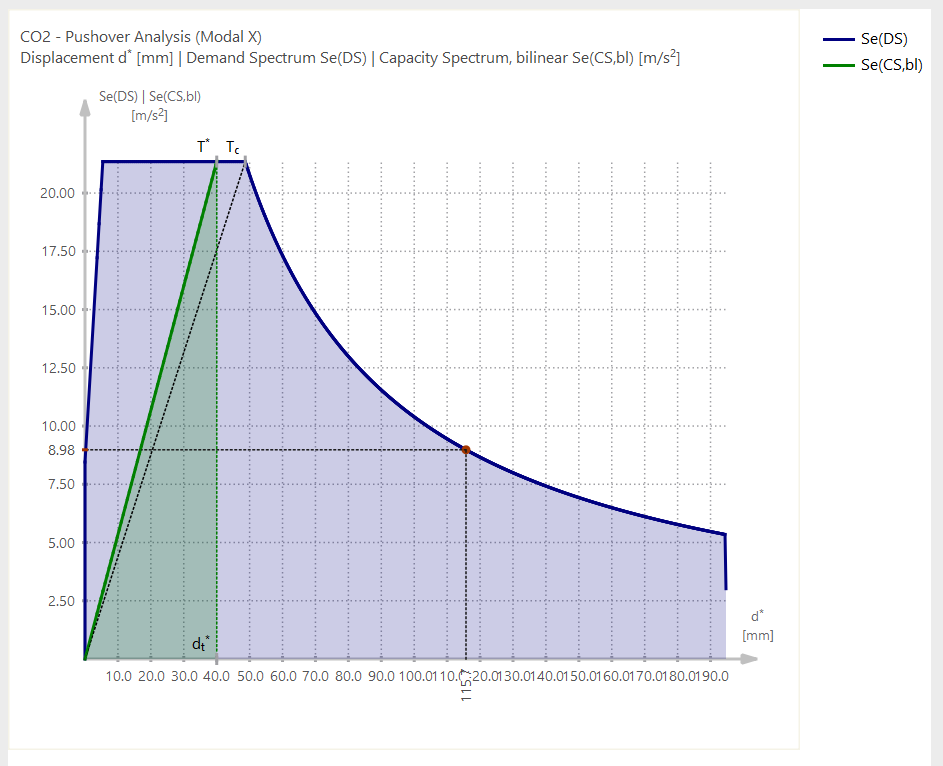
\includegraphics[width=0.6\textwidth]{Figures/cvd1.png}
\caption{Original Reference PGA \(a_{g,R} = 3.34 m/s^2\)}
\end{figure}


\begin{figure}
\centering
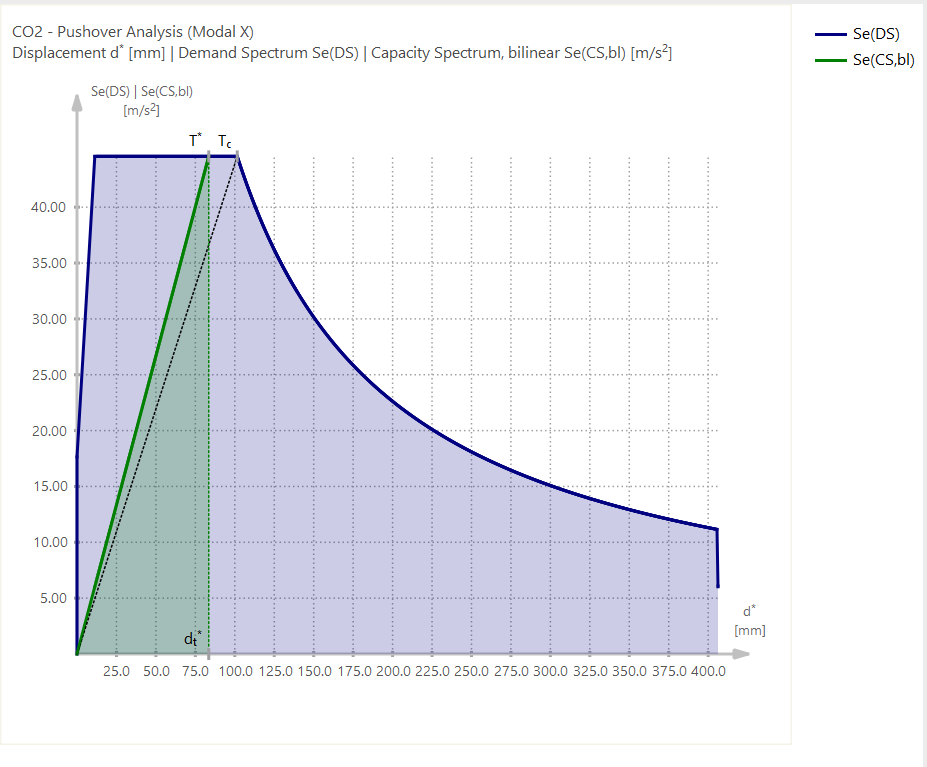
\includegraphics[width=0.6\textwidth]{Figures/cvd2.png}
\caption{Increased Reference PGA \(a_{g,R} = 10.00 m/s^2\)}
\end{figure}


\begin{figure}
\centering
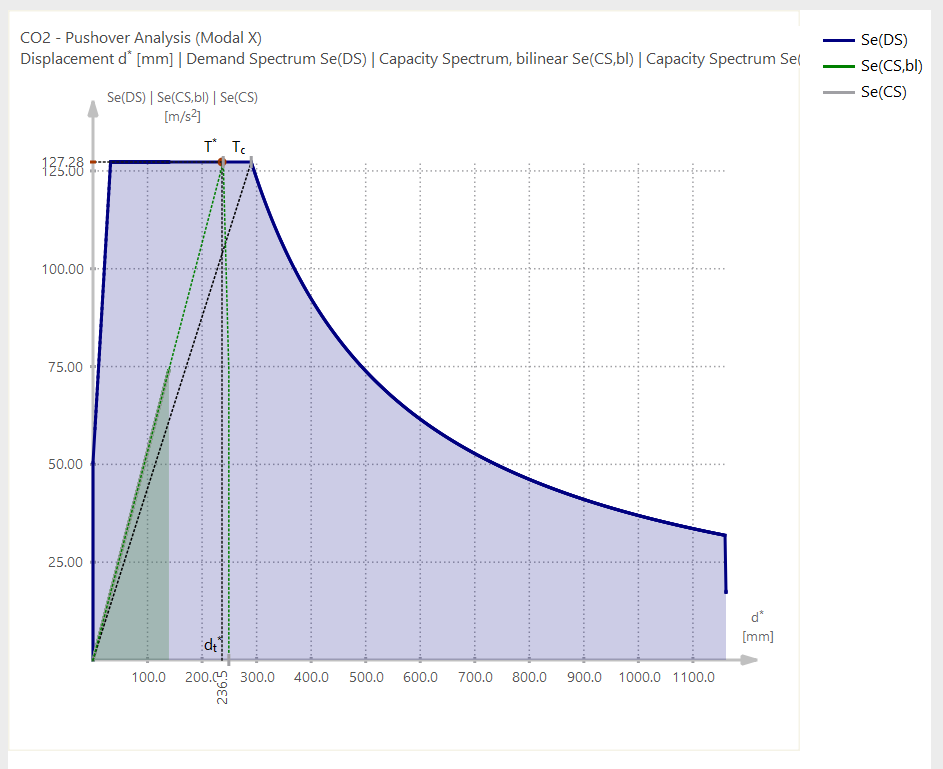
\includegraphics[width=0.6\textwidth]{Figures/cvd3.png}
\caption{Increased Reference PGA \(a_{g,R} = 15.00 m/s^2\)}
\end{figure}

\begin{figure}
\centering
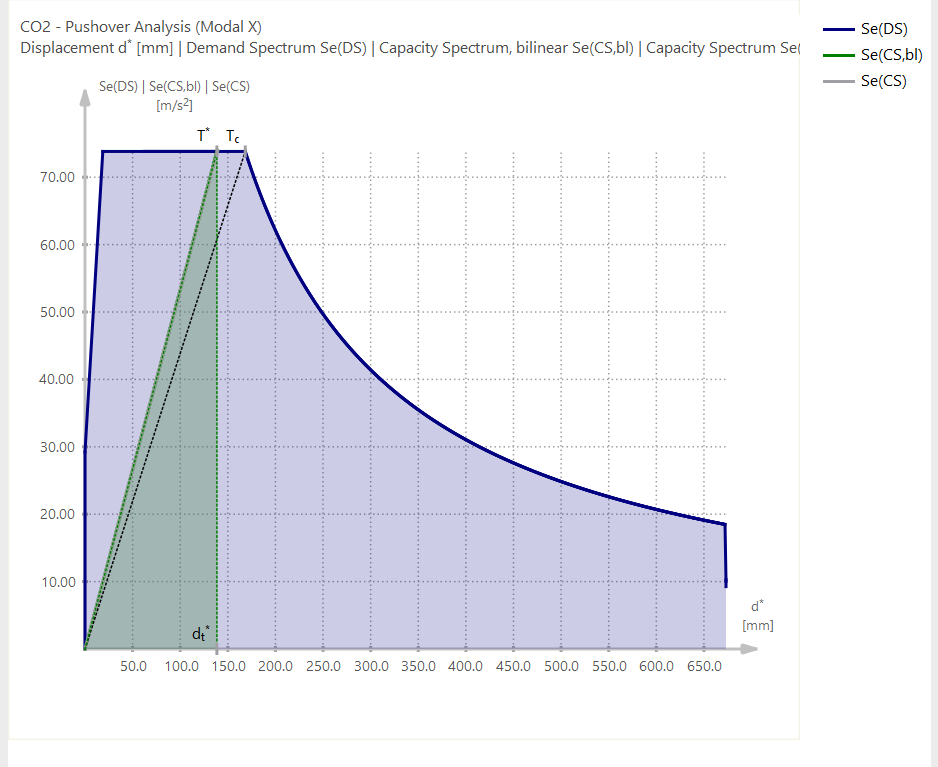
\includegraphics[width=0.6\textwidth]{Figures/cvd4.png}
\caption{Increased Reference PGA \(a_{g,R} = 11.60 m/s^2\), limit state}
\end{figure}

 \captionsetup{format=nocaption,aboveskip=0pt,belowskip=0pt}

Our structure is able to withstand the acceleration imposed by EN1998-1
standard within its elastic regime. According to the simulation no
plastic response is developed within failure.So different iterations
were done by adjusting the seismic demand to higher values by adjusting
the PGA. Upon further research, the conclusion that a more refined model
would be necessary in order to develop a plastic phase in the capacity
spectrum was reached. I would in fact be necessary to include a model of
the connections in order to correctly reproduce structural collapse,
whereas the current model can deform indefinitely. This was the
interpretation given to the following diagram, where Von Mises
equivalent stresses are plotted.

\begin{figure}
\centering
\pandocbounded{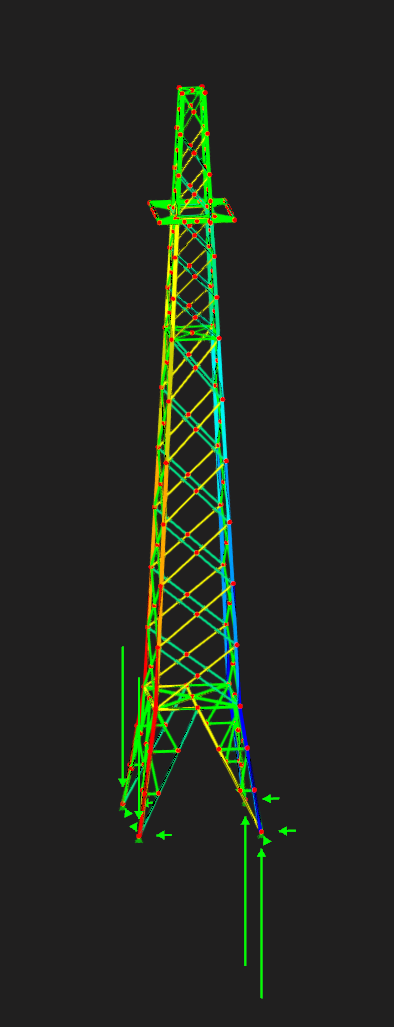
\includegraphics[keepaspectratio]{Figures/POA_no_plastic_phase.png}}
\caption{pushover\_no\_plastic}
\end{figure}

    \section{Section 3.c}\label{section-3.c}

According to EN1998-1-2005 section 4.3.3.2.1 a single mode approximation
is a viable option when the period of the chosen mode of vibration
satisfies the following conditions: \[
T_n<
\begin{cases}
4*T_C \\
2s
\end{cases}
\] In our design scenario \(T_C=0.3s\) and \(4*T_C=1.2s\). Mode 2 was
chosen for the analysis in X direction and respects the above mentioned
condition with \(T_2=0.27 s\). Mode 1 was chosen for the analysis in Y
direction with \(T_1=0.27 s\). No further load combinations are
therefore deemed necessary. On a more qualitative level, Mode 1 and 2
present a modal shape that maximize displacement at the top of the
structure in the main directions. The corresponding load patterns are
considered an appropriate choice in maximizing the overturning moment,
which is expected to be the most critical action for a cantilever beam
structure. Finally, the relatively high Effective Modal Mass Factor of
Mode 1 and 2 set at 0.44 (see table in Section 5 Part A) supports such
decision, especially since a single modal shape needs to be selected in
this analysis.

    \subsection{Section 4 - Time History
Analysis}\label{section-4---time-history-analysis}

A Time History Analysis was carried out as part of the seismic
assessment of the structure. Signal 1 was chosen from previously
processed data and the model was subjected to the derived accelerations
in the three principal directions.\\
As part of this analysis a limitation of the RFEM software was
encountered: the Stress-Analysis module did not support nonlinear
material behavior for members. As a consequence the analysis was carried
out in both bilinear and linear regimes, but stresses were computed for
linear regime. It is therefore implicitly assumed that the linear
behavior of the structure is sufficient to identify critical stresses
location.

The comparison of \textbf{maximum displacements} yielded the following
results:

\begin{longtable}[]{@{}ccccl@{}}
\toprule\noalign{}
DOF & Member & Material Bilinear & Material Linear & Description \\
\midrule\noalign{}
\endhead
\bottomrule\noalign{}
\endlastfoot
X & 313 & -83.5 mm & -83.3 mm & Top of the tower \\
Y & 365 & 87.0 mm & 86.3 mm & Antenna on mounting bracket \\
Z & 329 & -19.3 mm & 17.9 mm & Horizontal Bracing (2nd order) \\
\(\phi_x\) & 365 & 41.7 mrad & 41.0 mrad & Antenna on mounting
bracket \\
\(\phi_y\) & 329 & -18.4 mrad & 17.5 mrad & Horizontal Bracing (2nd
order) \\
\(\phi_z\) & 119 & -70.3 mrad & -70.6 mrad & Strut in basal truss
(lowest) \\
\end{longtable}

\clearpage
\textbf{High-stress locations (most relevant)}:


\begin{longtable}[]{@{}
  >{\centering\arraybackslash}p{(\linewidth - 8\tabcolsep) * \real{0.1236}}
  >{\centering\arraybackslash}p{(\linewidth - 8\tabcolsep) * \real{0.1798}}
  >{\centering\arraybackslash}p{(\linewidth - 8\tabcolsep) * \real{0.2697}}
  >{\centering\arraybackslash}p{(\linewidth - 8\tabcolsep) * \real{0.2247}}
  >{\centering\arraybackslash}p{(\linewidth - 8\tabcolsep) * \real{0.2022}}@{}}
\toprule\noalign{}
\begin{minipage}[b]{\linewidth}\centering
Member No.
\end{minipage} & \begin{minipage}[b]{\linewidth}\centering
Location x {[}m{]}
\end{minipage} & \begin{minipage}[b]{\linewidth}\centering
Stress Existing {[}N/mm2{]}
\end{minipage} & \begin{minipage}[b]{\linewidth}\centering
Stress Limit {[}N/mm2{]}
\end{minipage} & \begin{minipage}[b]{\linewidth}\centering
Stress Ratio \(\eta\) {[}-{]}
\end{minipage} \\
\midrule\noalign{}
\endhead
\bottomrule\noalign{}
\endlastfoot
111 & 1.874 & 200.340 & 235.000 & 0.853 \\
117 & 0.000 & 201.047 & 235.000 & 0.856 \\
311 & 1.707 & 211.905 & 235.000 & 0.902 \\
312 & 0.000 & 215.914 & 235.000 & 0.919 \\
329 & 0.000 & 258.318 & 235.000 & 1.099 \\
331 & 1.354 & 258.399 & 235.000 & 1.100 \\
\end{longtable}

\begin{figure}
\centering
\pandocbounded{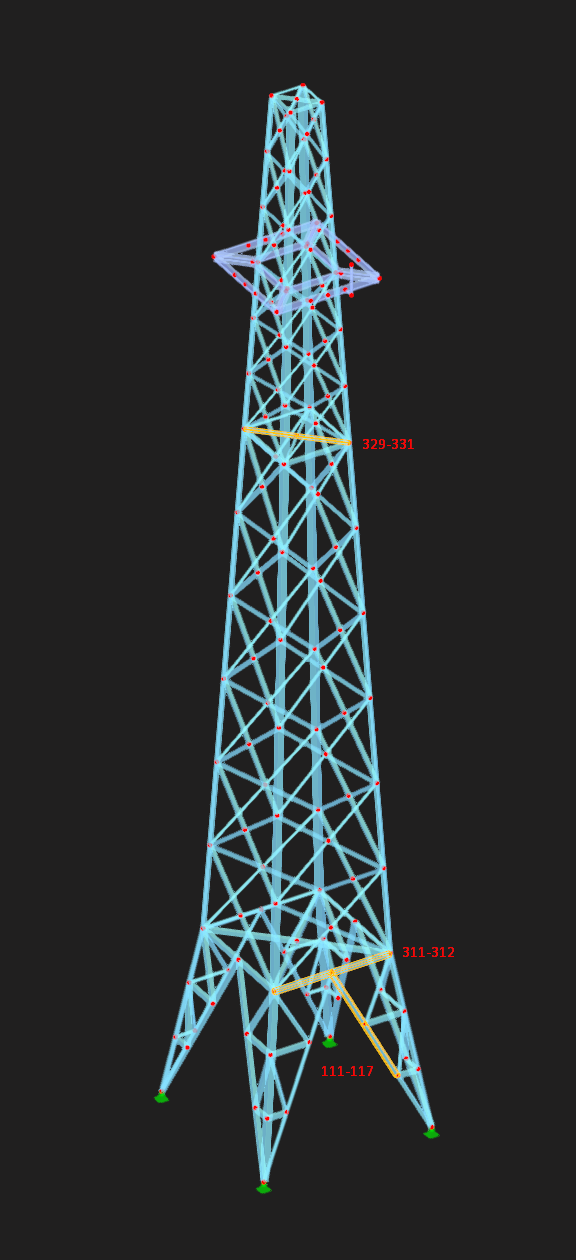
\includegraphics[keepaspectratio]{Figures/THA_critical_elements.png}}
\caption{THA - Critical Stresses Members}
\end{figure}

Displayed stresses were computed with Von Mises equivalent stresses
criterion. Comparing stresses with yielding stress values for the chosen
material shows that most critical excitation is located at the interface
between Members 329-331. At such locations the computed stresses due to
the ground acceleration provided by the timeseries (Signal 1) input in
the model exceed the limit stress of the material causing failure of the
structure. This finding is consistent with Spectral and Modal analysis
results. Mode 41, which excites precisely members 329-331 as shown in
the following figure, has in fact a period of \(0.065 s\) which closely
matches the peak frequency of the vertical component of the Elastic
Response Spectrum computed for the chosen signal.

\begin{figure}
\centering
\pandocbounded{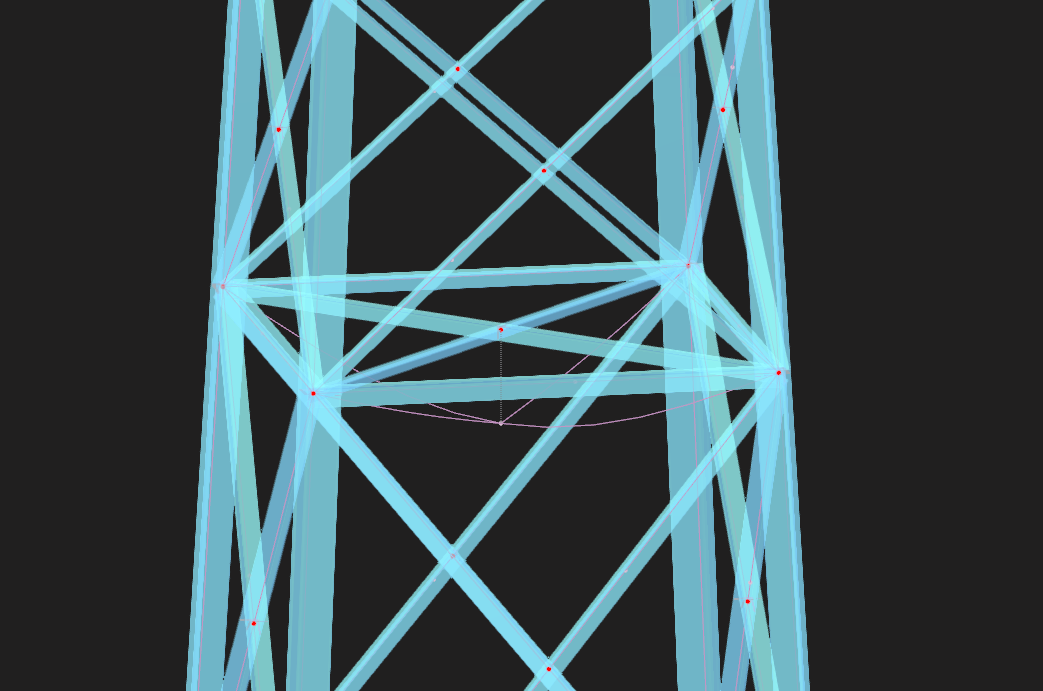
\includegraphics[keepaspectratio]{Figures/THA_def_mode41.png}}
\caption{THA\_mode41}
\end{figure}

\begin{figure}
\centering
\pandocbounded{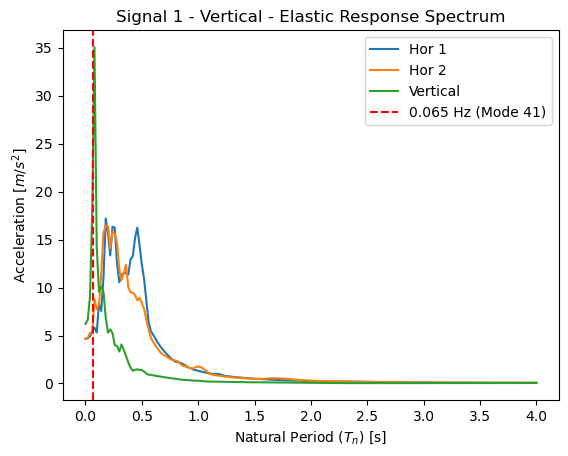
\includegraphics[keepaspectratio]{Figures/THA_signal1_mode41.png}}
\caption{THA\_signal1}
\end{figure}

In conclusion, the results of the Time Series Analyisis would hint
towards a vulnerability of the structure to vertical accelerations and
therefore inadequacy of the design to withstand seismic load. It is
however worth pointing out that the peak stress observed in members
329-331 is the result of a resonance between the spectral component
located at 15.38 Hz in Signal 1 and mode 41 of the structure. Given that
Signal 1 shows an unusually high peak when compared to the other signals
that were taken into consideration, this result may require further
examination of the validity and/or statistical relevance of Signal 1 and
the design may not need further refinement. If the signal were to be
considered relevant, the possible options to mitigate the problem would
include the use of stronger profiles for members 329-331 and/or damping
devices that would target displacements at the intersection of member
329-331. In both cases the analysis should be repeated as both options
may in principle affect the dynamic behavior of the structure,
potentially relocating the critical section.

    \section{Section 5 - Response Spectrum
Analysis}\label{section-5---response-spectrum-analysis}

\subsection{Part A}\label{part-a}

\captionsetup{format=plain, labelformat=empty, aboveskip=5pt,belowskip=5pt}
\begin{figure}
	\centering
	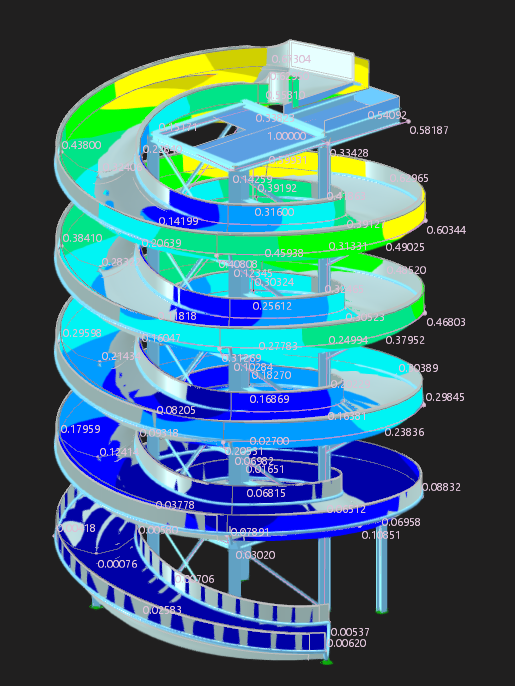
\includegraphics[height=0.8\textheight]{Figures/MA_1.png}
	\caption{Modal shape 1}
\end{figure}
\begin{figure}
	\centering
	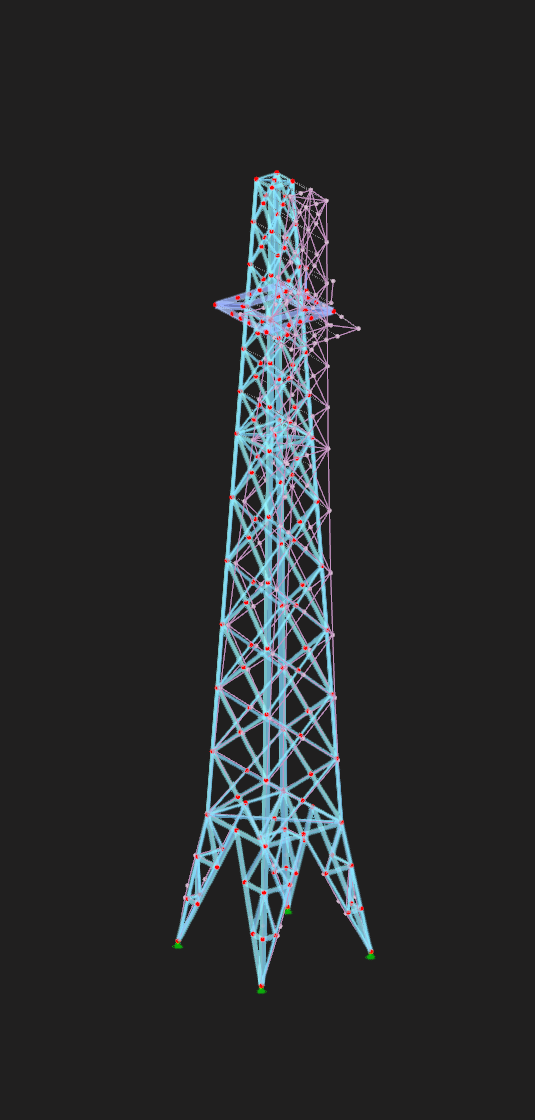
\includegraphics[height=0.8\textheight]{Figures/MA_2.png}
	\caption{Modal shape 2}
\end{figure}

\begin{figure}
	\centering
	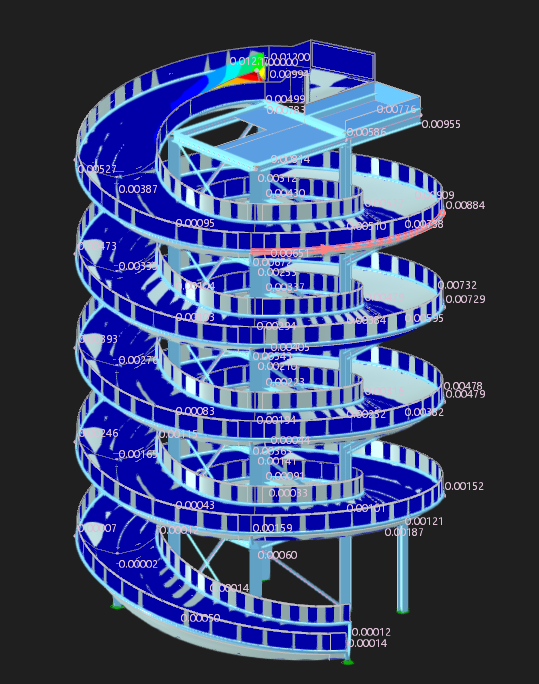
\includegraphics[height=0.8\textheight]{Figures/MA_3.png}
	\caption{Modal shape 3}
\end{figure}

\begin{figure}
	\centering
	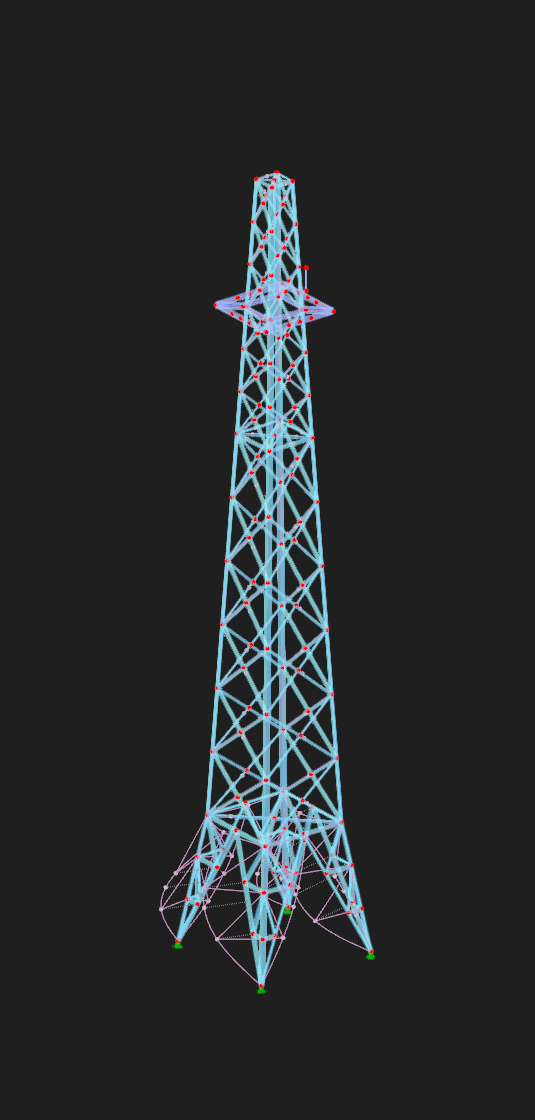
\includegraphics[height=0.8\textheight]{Figures/MA_4.png}
	\caption{Modal shape 4}
\end{figure}
\begin{figure}
	\centering
	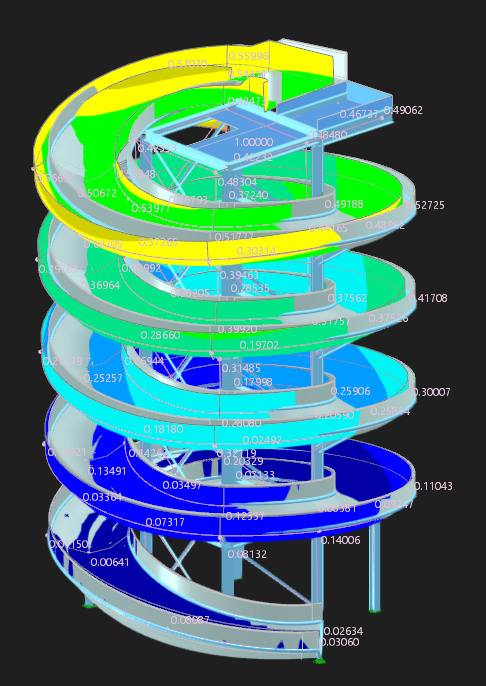
\includegraphics[height=0.8\textheight]{Figures/MA_5.png}
	\caption{Modal shape 5}
\end{figure}
 \captionsetup{format=nocaption,aboveskip=0pt,belowskip=0pt}

\clearpage
\begin{longtable}[]{@{}
  >{\raggedright\arraybackslash}p{(\linewidth - 16\tabcolsep) * \real{0.1111}}
  >{\raggedright\arraybackslash}p{(\linewidth - 16\tabcolsep) * \real{0.1111}}
  >{\raggedright\arraybackslash}p{(\linewidth - 16\tabcolsep) * \real{0.1111}}
  >{\raggedright\arraybackslash}p{(\linewidth - 16\tabcolsep) * \real{0.1111}}
  >{\raggedright\arraybackslash}p{(\linewidth - 16\tabcolsep) * \real{0.1111}}
  >{\raggedright\arraybackslash}p{(\linewidth - 16\tabcolsep) * \real{0.1111}}
  >{\raggedright\arraybackslash}p{(\linewidth - 16\tabcolsep) * \real{0.1111}}
  >{\raggedright\arraybackslash}p{(\linewidth - 16\tabcolsep) * \real{0.1111}}
  >{\raggedright\arraybackslash}p{(\linewidth - 16\tabcolsep) * \real{0.1111}}@{}}
\toprule\noalign{}
\begin{minipage}[b]{\linewidth}\raggedright
Mode Nr
\end{minipage} & \begin{minipage}[b]{\linewidth}\raggedright
NF
\end{minipage} & \begin{minipage}[b]{\linewidth}\raggedright
Modal Mass
\end{minipage} & \begin{minipage}[b]{\linewidth}\raggedright
EMM X
\end{minipage} & \begin{minipage}[b]{\linewidth}\raggedright
EMM Y
\end{minipage} & \begin{minipage}[b]{\linewidth}\raggedright
EMM Z
\end{minipage} & \begin{minipage}[b]{\linewidth}\raggedright
EMM \(\phi_x\)
\end{minipage} & \begin{minipage}[b]{\linewidth}\raggedright
EMM \(\phi_y\)
\end{minipage} & \begin{minipage}[b]{\linewidth}\raggedright
EMM \(\phi_z\)
\end{minipage} \\
\midrule\noalign{}
\endhead
\bottomrule\noalign{}
\endlastfoot
1 & 3.667 & 1683.0 & 89.4 & 3848.9 & 0.0 & 364106.00 & 7104.35 & 0.00 \\
2 & 3.668 & 1682.2 & 3849.0 & 89.4 & 0.0 & 7102.31 & 364118.00 & 0.01 \\
3 & 5.839 & 449.9 & 428.6 & 217.7 & 0.0 & 28487.50 & 41881.80 & 0.00 \\
4 & 5.839 & 450.0 & 217.7 & 428.5 & 0.0 & 41887.40 & 28488.40 & 0.00 \\
5 & 5.855 & 544.5 & 0.0 & 0.0 & 0.0 & 0.00 & 0.00 & 0.00 \\
28 & 12.026 & 0 & 0 & 0 & 0.4 & 0.16 & 10369 & 0 \\
55 & 18.897 & 0 & 0.5 & 0.4 & 18.92 & 0.03 & 10792.4 & 0 \\
84 & 25.518 & 0.2 & 0 & 3684.2 & 0.61 & 16.97 & 13.18 & 0 \\
\end{longtable}

\begin{longtable}[]{@{}
  >{\raggedright\arraybackslash}p{(\linewidth - 14\tabcolsep) * \real{0.1250}}
  >{\raggedright\arraybackslash}p{(\linewidth - 14\tabcolsep) * \real{0.1250}}
  >{\raggedright\arraybackslash}p{(\linewidth - 14\tabcolsep) * \real{0.1250}}
  >{\raggedright\arraybackslash}p{(\linewidth - 14\tabcolsep) * \real{0.1250}}
  >{\raggedright\arraybackslash}p{(\linewidth - 14\tabcolsep) * \real{0.1250}}
  >{\raggedright\arraybackslash}p{(\linewidth - 14\tabcolsep) * \real{0.1250}}
  >{\raggedright\arraybackslash}p{(\linewidth - 14\tabcolsep) * \real{0.1250}}
  >{\raggedright\arraybackslash}p{(\linewidth - 14\tabcolsep) * \real{0.1250}}@{}}
\toprule\noalign{}
\begin{minipage}[b]{\linewidth}\raggedright
Mode Nr
\end{minipage} & \begin{minipage}[b]{\linewidth}\raggedright
NF
\end{minipage} & \begin{minipage}[b]{\linewidth}\raggedright
Factor X
\end{minipage} & \begin{minipage}[b]{\linewidth}\raggedright
Factor Y
\end{minipage} & \begin{minipage}[b]{\linewidth}\raggedright
Factor Z
\end{minipage} & \begin{minipage}[b]{\linewidth}\raggedright
Factor \(\phi_X\)
\end{minipage} & \begin{minipage}[b]{\linewidth}\raggedright
Factor \(\phi_Y\)
\end{minipage} & \begin{minipage}[b]{\linewidth}\raggedright
Factor \(\phi_Z\)
\end{minipage} \\
\midrule\noalign{}
\endhead
\bottomrule\noalign{}
\endlastfoot
1 & 3.667 & 0.010 & 0.440 & 0.000 & 0.510 & 0.010 & 0.000 \\
2 & 3.668 & 0.440 & 0.010 & 0.000 & 0.010 & 0.510 & 0.000 \\
3 & 5.839 & 0.049 & 0.025 & 0.000 & 0.040 & 0.059 & 0.000 \\
4 & 5.839 & 0.025 & 0.049 & 0.000 & 0.059 & 0.040 & 0.000 \\
5 & 5.855 & 0.000 & 0.000 & 0.000 & 0.000 & 0.000 & 0.000 \\
28 & 12.026 & 0 & 0 & 0 & 0 & 0 & 0.335 \\
55 & 18.897 & 0 & 0 & 0 & 0 & 0 & 0.349 \\
84 & 25.518 & 0 & 0.421 & 0 & 0 & 0 & 0 \\
\end{longtable}

Inspecting the results of the modal analysis for 500 modes, the most
relevant modes are mode 1 and 2 with a modal mass factor of 0.44 in for
translational y and x direction respectively. These modes are also
relevant to describe the global bending behavior of the truss structure
with a modal mass factor of 0.51 in rotational x-direction and
y-direction respectively. The similarity in properties between the two
modes is to be expected as a result of the highly symmetric geometry of
the structure. Mode 3 and 4 concern deformations of the basal supports
of the truss, however their contribution is secondarily relevant to
describe the dynamic behavior of the structure and may be arguably
excluded from the analysis. In fact, EN1998-1 recommends a threshold of
0.05 for the participation ratio in the selection of modes as part of
the truncation process, however 0.049 is hereby regarded as a relatively
high contribution for a single mode. Mode 5 is interpreted as a
numerical artifact and therefore irrelevant. The first 5 modes are
highly inadequate to describe the deformation of the structure in
vertical and torsional directions (translation and rotation about z).
The most relevant mode for the former direction would be mode 84 (with a
mass participation ratio (z) of 0.421) while modes 28 and 55 are the
main contributors for the latter direction (counter-clockwise and
clockwise torsion) with mass participation ratio of 0.339 and 0.349
respectively.

\subsection{Part B}\label{part-b}

As mentioned in relation to Time History Analysis, due to RFEM features,
maximum displacements were computed for both linear and nonlinear
material, while stress-analysis was carried out for linear material
only.

CQC method was preferred to the SRSS rule to combine structural modes.
This choice was based on the robustness of CQC when dealing with modes
of vibration close in frequency. Although the case at hand did not
specifically require such attention CQC was the preferred choice as more
reliable and advanced modelling option. Moreover a damping ratio of 5\%
was taken as a realistic assumption for all modes, setting the domain
within the range of applicability of the CQC method. Given the EN1998-1
spectra wide band range CQC was also deemed more appropriate to the
specific design situation. SRSS was in turn selected to combined
different directional seismic components. This method was preferred to
the absolute sum method, which was deemed over-conservative, and to the
scaled sum method, which was discarded for its questionable approach to
modelling the real physical relation among seismic components from
different directions.

\begin{longtable}[]{@{}
  >{\centering\arraybackslash}p{(\linewidth - 8\tabcolsep) * \real{0.2000}}
  >{\centering\arraybackslash}p{(\linewidth - 8\tabcolsep) * \real{0.2000}}
  >{\centering\arraybackslash}p{(\linewidth - 8\tabcolsep) * \real{0.2000}}
  >{\centering\arraybackslash}p{(\linewidth - 8\tabcolsep) * \real{0.2000}}
  >{\raggedright\arraybackslash}p{(\linewidth - 8\tabcolsep) * \real{0.2000}}@{}}
\toprule\noalign{}
\begin{minipage}[b]{\linewidth}\centering
DOF
\end{minipage} & \begin{minipage}[b]{\linewidth}\centering
Member
\end{minipage} & \begin{minipage}[b]{\linewidth}\centering
Material Bilinear
\end{minipage} & \begin{minipage}[b]{\linewidth}\centering
Material Linear
\end{minipage} & \begin{minipage}[b]{\linewidth}\raggedright
Description
\end{minipage} \\
\midrule\noalign{}
\endhead
\bottomrule\noalign{}
\endlastfoot
X & 321 & 61.3 mm & 61.3 mm & Top of tower \\
Y & 309 & 61.3 mm & 61.3 mm & Top of tower \\
Z & 333 & 11.5 mm & 11.5 mm & Horizontal Bracing (1st order) \\
\(\phi_x\) & 239 & 12.0 mrad & 12.0 mrad & Strut in basal truss (2nd
from bottom) \\
\(\phi_y\) & 177 & 12.0 mrad & 12.0 mrad & Strut in basal truss (2nd
from bottom) \\
\(\phi_z\) & 181 & 36.5 mrad & 36.5 mrad & Strut in basal truss
(lowest) \\
\end{longtable}

\textbf{High-stress locations (most relevant)}:

\begin{longtable}[]{@{}
  >{\centering\arraybackslash}p{(\linewidth - 8\tabcolsep) * \real{0.1236}}
  >{\centering\arraybackslash}p{(\linewidth - 8\tabcolsep) * \real{0.1798}}
  >{\centering\arraybackslash}p{(\linewidth - 8\tabcolsep) * \real{0.2697}}
  >{\centering\arraybackslash}p{(\linewidth - 8\tabcolsep) * \real{0.2247}}
  >{\centering\arraybackslash}p{(\linewidth - 8\tabcolsep) * \real{0.2022}}@{}}
\toprule\noalign{}
\begin{minipage}[b]{\linewidth}\centering
Member No.
\end{minipage} & \begin{minipage}[b]{\linewidth}\centering
Location x {[}m{]}
\end{minipage} & \begin{minipage}[b]{\linewidth}\centering
Stress Existing {[}N/mm2{]}
\end{minipage} & \begin{minipage}[b]{\linewidth}\centering
Stress Limit {[}N/mm2{]}
\end{minipage} & \begin{minipage}[b]{\linewidth}\centering
Stress Ratio \(\eta\) {[}-{]}
\end{minipage} \\
\midrule\noalign{}
\endhead
\bottomrule\noalign{}
\endlastfoot
81 & 1.183 & 117.558 & 235.000 & 0.500 \\
84 & 0.000 & 119.666 & 235.000 & 0.509 \\
143 & 1.183 & 117.466 & 235.000 & 0.500 \\
146 & 0.000 & 119.577 & 235.000 & 0.509 \\
205 & 1.183 & 117.314 & 235.000 & 0.499 \\
208 & 0.000 & 119.421 & 235.000 & 0.508 \\
267 & 1.183 & 117.533 & 235.000 & 0.500 \\
270 & 0.000 & 119.641 & 235.000 & 0.509 \\
311 & 1.707 & 126.505 & 235.000 & 0.538 \\
312 & 0.000 & 126.471 & 235.000 & 0.538 \\
315 & 1.707 & 126.560 & 235.000 & 0.539 \\
316 & 0.000 & 126.524 & 235.000 & 0.538 \\
319 & 1.707 & 126.516 & 235.000 & 0.538 \\
320 & 0.000 & 126.471 & 235.000 & 0.538 \\
323 & 1.707 & 126.512 & 235.000 & 0.538 \\
324 & 0.000 & 126.444 & 235.000 & 0.538 \\
\end{longtable}

\begin{figure}
\centering
\pandocbounded{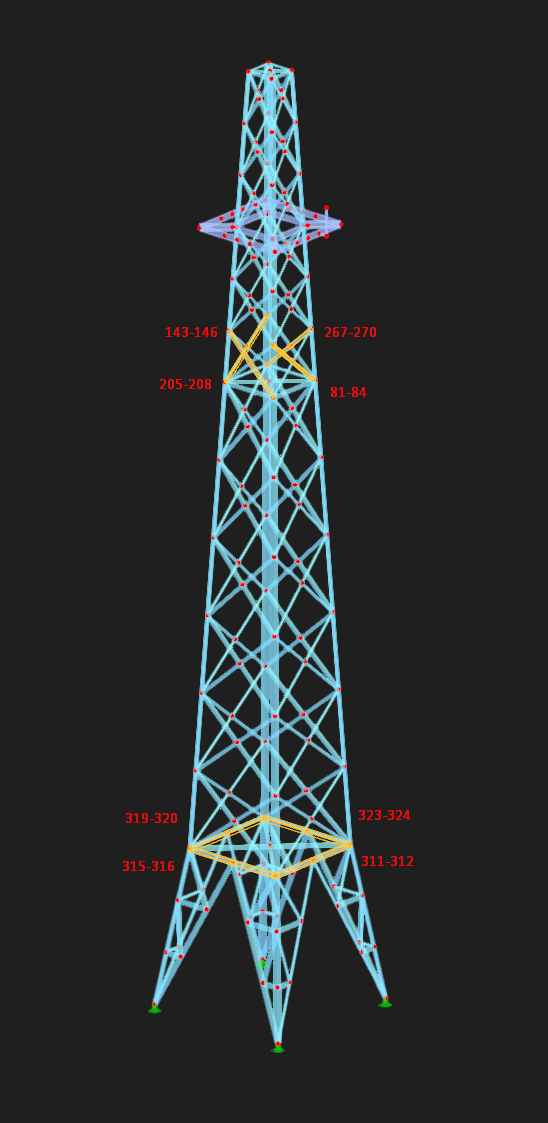
\includegraphics[keepaspectratio]{Figures/RSA_critical_elements.png}}
\caption{RSA - Critical Stresses Members}
\end{figure}

As shown by the previous figure, the elements that present the highest
stress ratio can be collected in two sets. As it could be expected there
is only partial correspondence between the critical cross sections
obtained from Response Spectrum Analysis and the Time History Analysis.
It is first interesting to point out that the RSA results are completely
symmetric whereas the THA are not. This is consistent with the spectra
in the x and y direction being equal as prescribed by EN1998-1 in the
RSA, as opposed to the recorded accelerogram considered for the THA.
Even if the input spectra differ significantly, elements 311-312 appear
as critical sections in both analysis. This is not surprising as those
members are at the interface between the basal part and the upper part
of the structure, which is where the load is transferred from the main
truss structure to the support trusses. However it is apparent how the
RSA produces significantly lower stress-ratios. Finally, the set of
elements located in the upper part of the structure
(81,84,143,146,205,208,267,270) do not find correspondence in the THA
results. Relatively to the RSA results alone, this is explained by a
higher relevance of horizontal excitations in the RSA. In relation to
the THA, the dominance of vertical accelerations make these members
irrelevant compared to others.

\subsection{Part C}\label{part-c}

An incremental number of modes was considered in order to obtain a 90\%
cumulative sum of modal participation factors, as recommended by
EN1998-1.

\begin{longtable}[]{@{}
  >{\centering\arraybackslash}p{(\linewidth - 12\tabcolsep) * \real{0.1429}}
  >{\centering\arraybackslash}p{(\linewidth - 12\tabcolsep) * \real{0.1429}}
  >{\centering\arraybackslash}p{(\linewidth - 12\tabcolsep) * \real{0.1429}}
  >{\centering\arraybackslash}p{(\linewidth - 12\tabcolsep) * \real{0.1429}}
  >{\centering\arraybackslash}p{(\linewidth - 12\tabcolsep) * \real{0.1429}}
  >{\centering\arraybackslash}p{(\linewidth - 12\tabcolsep) * \real{0.1429}}
  >{\centering\arraybackslash}p{(\linewidth - 12\tabcolsep) * \real{0.1429}}@{}}
\toprule\noalign{}
\begin{minipage}[b]{\linewidth}\centering
N Modes
\end{minipage} & \begin{minipage}[b]{\linewidth}\centering
X
\end{minipage} & \begin{minipage}[b]{\linewidth}\centering
Y
\end{minipage} & \begin{minipage}[b]{\linewidth}\centering
Z
\end{minipage} & \begin{minipage}[b]{\linewidth}\centering
\(\phi_x\)
\end{minipage} & \begin{minipage}[b]{\linewidth}\centering
\(\phi_y\)
\end{minipage} & \begin{minipage}[b]{\linewidth}\centering
\(\phi_z\)
\end{minipage} \\
\midrule\noalign{}
\endhead
\bottomrule\noalign{}
\endlastfoot
10 & 52.44 \% & 52.40 \% & 0.28 \% & 61.85 \% & 61.86 \% & 5.69 \% \\
50 & 72.97 \% & 73.01 \% & 2.26 \% & 70.04 \% & 70.02 \% & 43.17 \% \\
100 & 96.24 \% & 96.31 \% & 46.66 \% & 92.35 \% & 92.24 \% & 83.58 \% \\
500 & 98.01 \% & 98.01 \% & 79.69 \% & 96.39 \% & 96.40 \% & 93.43 \% \\
\end{longtable}

The Response Spectrum Analysis was carried out with a 500 mode
approximation. It is worth noting that the summation of mass ratios in
the Z direction does not meet the recommended value. The main reason
behind such truncation decision was ensuring computational manageability
of the model. From a physical point of view, this modelling choice
should not impact significantly the results of the analysis, since the
(cantilever) beam-like behavior of the structure should guarantee high
resistance in the axial direction. Moreover, the dominant excitations
imposed by EN1998-1 are horizontally directed, which further supports
the implemented assumption, however this vulnerability should not go
overlooked when vertical accelerations are relevant, as shown by the
results of Time History Analysis where mode 41 proved to be determining.

Elaborating further on the sensitivity of the results to the number of
modes used in the analysis, it can be observed by comparing the previous
and the following table that no difference is encountered in the
numerical results between 50, 100 and 500 (disclaimer: Member 115 is a
symmetric counterpart of Member 239). A small numerical difference is
instead recorded between 10 and 50 modes approximation.

\begin{longtable}[]{@{}
  >{\centering\arraybackslash}p{(\linewidth - 12\tabcolsep) * \real{0.1429}}
  >{\centering\arraybackslash}p{(\linewidth - 12\tabcolsep) * \real{0.1429}}
  >{\centering\arraybackslash}p{(\linewidth - 12\tabcolsep) * \real{0.1429}}
  >{\centering\arraybackslash}p{(\linewidth - 12\tabcolsep) * \real{0.1429}}
  >{\centering\arraybackslash}p{(\linewidth - 12\tabcolsep) * \real{0.1429}}
  >{\centering\arraybackslash}p{(\linewidth - 12\tabcolsep) * \real{0.1429}}
  >{\centering\arraybackslash}p{(\linewidth - 12\tabcolsep) * \real{0.1429}}@{}}
\toprule\noalign{}
\begin{minipage}[b]{\linewidth}\centering
N Modes
\end{minipage} & \begin{minipage}[b]{\linewidth}\centering
Max Disp. X
\end{minipage} & \begin{minipage}[b]{\linewidth}\centering
Max Disp. Y
\end{minipage} & \begin{minipage}[b]{\linewidth}\centering
Max Disp. Z
\end{minipage} & \begin{minipage}[b]{\linewidth}\centering
Max Disp. \(\phi_x\)
\end{minipage} & \begin{minipage}[b]{\linewidth}\centering
Max Disp. \(\phi_y\)
\end{minipage} & \begin{minipage}[b]{\linewidth}\centering
Max Disp. \(\phi_z\)
\end{minipage} \\
\midrule\noalign{}
\endhead
\bottomrule\noalign{}
\endlastfoot
10 & 61.4 mm Member No.~313 & 70.1 mm Member No.~365 & 11.5 mm Member
No.~365 & 25.5 mrad Member No.~365 & 11.9 mrad Member No.~301 & 36.4
mrad Member No.~119 \\
50 & 61.3 mm Member No.~313 & 61.3 mm Member No.~309 & 11.5 mm Member
No.~333 & 12.0 mrad Member No.~115 & 12.0 mrad Member No.~177 & 36.5
mrad Member No.~181 \\
100 & 61.3 mm Member No.~313 & 61.3 mm Member No.~309 & 11.5 mm Member
No.~333 & 12.0 mrad Member No.~239 & 12.0 mrad Member No.~177 & 36.5
mrad Member No.~181 \\
500 & 61.3 mm Member No.~313 & 61.3 mm Member No.~309 & 11.5 mm Member
No.~333 & 12.0 mrad Member No.~239 & 12.0 mrad Member No.~177 & 36.5
mrad Member No.~181 \\
\end{longtable}

\subsection{Part D}\label{part-d}

The structure is able to withstand the standardized seismic loads
prescribed by EN1998-1. The computed stress ratios are well within unity
check for all members. Additionally, no significant resonance was found.

    \section{Section 6 - Soil Structure
Interaction}\label{section-6---soil-structure-interaction}

A preliminary design of the foundation was carried out as a first step.
In order to match the double symmetry of the structure a square slab was
the preferred choice. The dimensions were derived based on the maximum
overturning moment developed during the pushover analysis, corresponding
to 2811 kNm. Within the scope of approximation, a linear stress
distribution was assumed along the length (maximum soil stress il
reached on the left side and no lift was considered on the right side)
and such distribution was assumed to be constant along width. An
arbitrary depth of 0.3 m was consider a valid first guess based on a
similar example in the study material.

Equilibrium: \(M_{pushover} = (\frac{c_uL}{2}\cdot L)\cdot\frac{L}{6}\)

Dimensions: \(L = B = \sqrt[3]{\frac{12*M_{pushover}}{c_u}}=8.77m\)

\begin{figure}
\centering
\pandocbounded{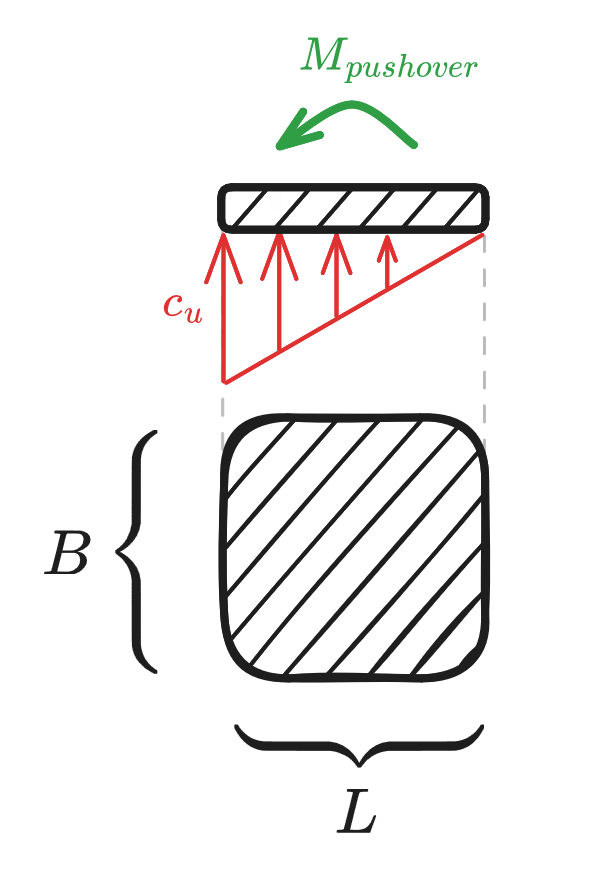
\includegraphics[width=0.22\textwidth]{Figures/SSI_foundation_design.png}}
\caption{foundation\_design}
\end{figure}

\subsection{Part A - Frequency Dependent Soil Stiffness
Matrix}\label{part-a---frequency-dependent-soil-stiffness-matrix}

    \begin{tcolorbox}[breakable, size=fbox, boxrule=1pt, pad at break*=1mm,colback=cellbackground, colframe=cellborder]
\prompt{In}{incolor}{3}{\boxspacing}
\begin{Verbatim}[commandchars=\\\{\}]
\PY{c+c1}{\PYZsh{} Soil Properties (indipendent of Student Number)}
\PY{n}{nu} \PY{o}{=} \PY{l+m+mf}{0.33}      \PY{c+c1}{\PYZsh{}[\PYZhy{}] Poisson Ratio}
\PY{n}{c\PYZus{}u} \PY{o}{=} \PY{l+m+mf}{50e3}     \PY{c+c1}{\PYZsh{}[Pa] Undrained Shear Strength}
\PY{n}{v\PYZus{}s} \PY{o}{=} \PY{l+m+mi}{160}      \PY{c+c1}{\PYZsh{}[m/s] Velocity of shear waves in soil}
\PY{n}{rho} \PY{o}{=} \PY{l+m+mi}{1800}     \PY{c+c1}{\PYZsh{}[kg/m\PYZca{}3] Soil Density}
\PY{n}{beta} \PY{o}{=} \PY{l+m+mf}{0.05}    \PY{c+c1}{\PYZsh{}[\PYZhy{}] Soil hysteretic (material) damping (arbitrarily chosen)}

\PY{c+c1}{\PYZsh{} Foundation dimensions (rectangular slab shallow foundation)}
\PY{n}{side\PYZus{}x} \PY{o}{=} \PY{n}{side\PYZus{}y} \PY{o}{=} \PY{l+m+mf}{8.77} \PY{c+c1}{\PYZsh{}[m] As a first implementation the slab is as large as the base of the tower}
\PY{n}{depth} \PY{o}{=} \PY{l+m+mf}{0.3} \PY{c+c1}{\PYZsh{}[m] height of foundation}

\PY{c+c1}{\PYZsh{} Structure}
\PY{c+c1}{\PYZsh{}\PYZsh{} Modal parameters from RFEM model (mode 2)}
\PY{n}{omega} \PY{o}{=} \PY{l+m+mf}{23.047} \PY{c+c1}{\PYZsh{}[rad/s] Frequency of interest (Mode 2 \PYZhy{} Main mode in X direction)}
\end{Verbatim}
\end{tcolorbox}

    The frequency dependent dynamic stiffness matrix was derived according
to the model proposed for a surface foundation on a homogenous half
space as per Gazetas, G. (1991).

\begin{itemize}
\tightlist
\item
  Citation: Gazetas, G. 1991. Formulas and charts for impedances of
  surface and embedded foundations. Journal of Geotechnical Engineering,
  117(9), 1363--1381.
  https://doi.org/10.1061/(asce)0733-9410(1991)117:9(1363)
\end{itemize}

    \begin{tcolorbox}[breakable, size=fbox, boxrule=1pt, pad at break*=1mm,colback=cellbackground, colframe=cellborder]
\prompt{In}{incolor}{4}{\boxspacing}
\begin{Verbatim}[commandchars=\\\{\}]
\PY{n}{L} \PY{o}{=} \PY{n}{side\PYZus{}x}\PY{o}{/}\PY{l+m+mi}{2}                                  \PY{c+c1}{\PYZsh{}[m] Half\PYZhy{}length between center of the circumscribed rectangle and side X\PYZhy{}direction (major direction)}
\PY{n}{B} \PY{o}{=} \PY{n}{side\PYZus{}y}\PY{o}{/}\PY{l+m+mi}{2}                                  \PY{c+c1}{\PYZsh{}[m] Half\PYZhy{}width between center of the circumscribed rectangle and side Y\PYZhy{}direction (minor direction)}
\PY{n}{A\PYZus{}b} \PY{o}{=} \PY{n}{side\PYZus{}x}\PY{o}{*}\PY{n}{side\PYZus{}y}                           \PY{c+c1}{\PYZsh{}[m] Foundation surface area}
\PY{n}{I\PYZus{}bx} \PY{o}{=} \PY{n}{side\PYZus{}x}\PY{o}{*}\PY{n}{side\PYZus{}y}\PY{o}{*}\PY{o}{*}\PY{l+m+mi}{3}\PY{o}{/}\PY{l+m+mi}{12}                    \PY{c+c1}{\PYZsh{}[m\PYZca{}4] Area moment of inertia about x\PYZhy{}axis}
\PY{n}{I\PYZus{}by} \PY{o}{=} \PY{n}{side\PYZus{}x}\PY{o}{*}\PY{o}{*}\PY{l+m+mi}{3}\PY{o}{*}\PY{n}{side\PYZus{}y}\PY{o}{/}\PY{l+m+mi}{12}                    \PY{c+c1}{\PYZsh{}[m\PYZca{}4] Area moment of inertia about y\PYZhy{}axis}
\PY{n}{I\PYZus{}bz} \PY{o}{=} \PY{n}{side\PYZus{}x}\PY{o}{*}\PY{n}{side\PYZus{}y}\PY{o}{*}\PY{p}{(}\PY{n}{side\PYZus{}x}\PY{o}{*}\PY{o}{*}\PY{l+m+mi}{2}\PY{o}{+}\PY{n}{side\PYZus{}y}\PY{o}{*}\PY{o}{*}\PY{l+m+mi}{2}\PY{p}{)}\PY{o}{/}\PY{l+m+mi}{12} \PY{c+c1}{\PYZsh{}[m\PYZca{}4] Area moment of inertia about z\PYZhy{}axis}
\PY{n}{G} \PY{o}{=} \PY{n}{c\PYZus{}u}                                       \PY{c+c1}{\PYZsh{}[Pa] Shear modulus}
\PY{n}{v\PYZus{}la} \PY{o}{=} \PY{l+m+mf}{3.4}\PY{o}{*}\PY{n}{v\PYZus{}s}\PY{o}{/}\PY{p}{(}\PY{n}{np}\PY{o}{.}\PY{n}{pi}\PY{o}{*}\PY{p}{(}\PY{l+m+mi}{1}\PY{o}{\PYZhy{}}\PY{n}{nu}\PY{p}{)}\PY{p}{)}                 \PY{c+c1}{\PYZsh{}[m/s] Lymer\PYZsq{}s analog wave velocity (formula from cited paper)}
\PY{n}{chi} \PY{o}{=} \PY{n}{A\PYZus{}b}\PY{o}{/}\PY{p}{(}\PY{l+m+mi}{4}\PY{o}{*}\PY{n}{L}\PY{o}{*}\PY{o}{*}\PY{l+m+mi}{2}\PY{p}{)}                            \PY{c+c1}{\PYZsh{}[\PYZhy{}] Parameter from cited paper\PYZsq{}\PYZdq{}Part B \PYZhy{} Notebook (Answers 3\PYZhy{}6).ipynb\PYZdq{}}

\PY{n+nb}{print}\PY{p}{(}\PY{l+s+s2}{\PYZdq{}}\PY{l+s+se}{\PYZbs{}n}\PY{l+s+s2}{INPUT RECAP:}\PY{l+s+s2}{\PYZdq{}}\PY{p}{)}
\PY{n+nb}{print}\PY{p}{(}\PY{l+s+sa}{f}\PY{l+s+s2}{\PYZdq{}}\PY{l+s+s2}{L: }\PY{l+s+si}{\PYZob{}}\PY{n}{L}\PY{l+s+si}{:}\PY{l+s+s2}{.3e}\PY{l+s+si}{\PYZcb{}}\PY{l+s+s2}{ m}\PY{l+s+s2}{\PYZdq{}}\PY{p}{)}
\PY{n+nb}{print}\PY{p}{(}\PY{l+s+sa}{f}\PY{l+s+s2}{\PYZdq{}}\PY{l+s+s2}{B: }\PY{l+s+si}{\PYZob{}}\PY{n}{B}\PY{l+s+si}{:}\PY{l+s+s2}{.3e}\PY{l+s+si}{\PYZcb{}}\PY{l+s+s2}{ m}\PY{l+s+s2}{\PYZdq{}}\PY{p}{)}
\PY{n+nb}{print}\PY{p}{(}\PY{l+s+sa}{f}\PY{l+s+s2}{\PYZdq{}}\PY{l+s+s2}{A\PYZus{}b: }\PY{l+s+si}{\PYZob{}}\PY{n}{A\PYZus{}b}\PY{l+s+si}{:}\PY{l+s+s2}{.3e}\PY{l+s+si}{\PYZcb{}}\PY{l+s+s2}{ m}\PY{l+s+s2}{\PYZdq{}}\PY{p}{)}
\PY{n+nb}{print}\PY{p}{(}\PY{l+s+sa}{f}\PY{l+s+s2}{\PYZdq{}}\PY{l+s+s2}{I\PYZus{}bx: }\PY{l+s+si}{\PYZob{}}\PY{n}{I\PYZus{}bx}\PY{l+s+si}{:}\PY{l+s+s2}{.3e}\PY{l+s+si}{\PYZcb{}}\PY{l+s+s2}{ m\PYZca{}4}\PY{l+s+s2}{\PYZdq{}}\PY{p}{)}
\PY{n+nb}{print}\PY{p}{(}\PY{l+s+sa}{f}\PY{l+s+s2}{\PYZdq{}}\PY{l+s+s2}{I\PYZus{}by: }\PY{l+s+si}{\PYZob{}}\PY{n}{I\PYZus{}by}\PY{l+s+si}{:}\PY{l+s+s2}{.3e}\PY{l+s+si}{\PYZcb{}}\PY{l+s+s2}{ m\PYZca{}4}\PY{l+s+s2}{\PYZdq{}}\PY{p}{)}
\PY{n+nb}{print}\PY{p}{(}\PY{l+s+sa}{f}\PY{l+s+s2}{\PYZdq{}}\PY{l+s+s2}{I\PYZus{}bz: }\PY{l+s+si}{\PYZob{}}\PY{n}{I\PYZus{}bz}\PY{l+s+si}{:}\PY{l+s+s2}{.3e}\PY{l+s+si}{\PYZcb{}}\PY{l+s+s2}{ m\PYZca{}4}\PY{l+s+s2}{\PYZdq{}}\PY{p}{)}
\PY{n+nb}{print}\PY{p}{(}\PY{l+s+sa}{f}\PY{l+s+s2}{\PYZdq{}}\PY{l+s+s2}{G: }\PY{l+s+si}{\PYZob{}}\PY{n}{G}\PY{l+s+si}{:}\PY{l+s+s2}{.3e}\PY{l+s+si}{\PYZcb{}}\PY{l+s+s2}{ Pa}\PY{l+s+s2}{\PYZdq{}}\PY{p}{)}
\PY{n+nb}{print}\PY{p}{(}\PY{l+s+sa}{f}\PY{l+s+s2}{\PYZdq{}}\PY{l+s+s2}{v\PYZus{}la: }\PY{l+s+si}{\PYZob{}}\PY{n}{v\PYZus{}la}\PY{l+s+si}{:}\PY{l+s+s2}{.3e}\PY{l+s+si}{\PYZcb{}}\PY{l+s+s2}{ m/s}\PY{l+s+s2}{\PYZdq{}}\PY{p}{)}
\PY{n+nb}{print}\PY{p}{(}\PY{l+s+sa}{f}\PY{l+s+s2}{\PYZdq{}}\PY{l+s+s2}{chi: }\PY{l+s+si}{\PYZob{}}\PY{n}{chi}\PY{l+s+si}{:}\PY{l+s+s2}{.3e}\PY{l+s+si}{\PYZcb{}}\PY{l+s+s2}{ \PYZhy{}}\PY{l+s+s2}{\PYZdq{}}\PY{p}{)}

\PY{c+c1}{\PYZsh{}Static Stiffness}
\PY{n}{K\PYZus{}z} \PY{o}{=} \PY{p}{(}\PY{l+m+mi}{2}\PY{o}{*}\PY{n}{G}\PY{o}{*}\PY{n}{L}\PY{o}{/}\PY{p}{(}\PY{l+m+mi}{1}\PY{o}{\PYZhy{}}\PY{n}{nu}\PY{p}{)}\PY{p}{)}\PY{o}{*}\PY{p}{(}\PY{l+m+mf}{0.73}\PY{o}{+}\PY{l+m+mf}{1.54}\PY{o}{*}\PY{n}{chi}\PY{o}{*}\PY{o}{*}\PY{l+m+mf}{0.75}\PY{p}{)}
\PY{n}{K\PYZus{}y} \PY{o}{=} \PY{p}{(}\PY{l+m+mi}{2}\PY{o}{*}\PY{n}{G}\PY{o}{*}\PY{n}{L}\PY{o}{/}\PY{p}{(}\PY{l+m+mi}{2}\PY{o}{\PYZhy{}}\PY{n}{nu}\PY{p}{)}\PY{p}{)}\PY{o}{*}\PY{p}{(}\PY{l+m+mi}{2}\PY{o}{+}\PY{l+m+mf}{2.50}\PY{o}{*}\PY{n}{chi}\PY{o}{*}\PY{o}{*}\PY{l+m+mf}{0.85}\PY{p}{)}
\PY{n}{K\PYZus{}x} \PY{o}{=} \PY{n}{K\PYZus{}y} \PY{o}{\PYZhy{}} \PY{p}{(}\PY{l+m+mf}{0.2}\PY{o}{/}\PY{p}{(}\PY{l+m+mf}{0.75}\PY{o}{\PYZhy{}}\PY{n}{nu}\PY{p}{)}\PY{p}{)}\PY{o}{*}\PY{n}{G}\PY{o}{*}\PY{n}{L}\PY{o}{*}\PY{p}{(}\PY{l+m+mi}{1}\PY{o}{\PYZhy{}}\PY{p}{(}\PY{n}{B}\PY{o}{/}\PY{n}{L}\PY{p}{)}\PY{p}{)}
\PY{n}{K\PYZus{}rx} \PY{o}{=} \PY{p}{(}\PY{n}{G}\PY{o}{/}\PY{p}{(}\PY{l+m+mi}{1}\PY{o}{\PYZhy{}}\PY{n}{nu}\PY{p}{)}\PY{p}{)}\PY{o}{*}\PY{n}{I\PYZus{}bx}\PY{o}{*}\PY{o}{*}\PY{l+m+mf}{0.75}\PY{o}{*}\PY{p}{(}\PY{n}{L}\PY{o}{/}\PY{n}{B}\PY{p}{)}\PY{o}{*}\PY{o}{*}\PY{l+m+mf}{0.25}\PY{o}{*}\PY{p}{(}\PY{l+m+mf}{2.4}\PY{o}{+}\PY{l+m+mf}{0.5}\PY{o}{*}\PY{p}{(}\PY{n}{B}\PY{o}{/}\PY{n}{L}\PY{p}{)}\PY{p}{)}
\PY{n}{K\PYZus{}ry} \PY{o}{=} \PY{p}{(}\PY{l+m+mi}{3}\PY{o}{*}\PY{n}{G}\PY{o}{/}\PY{p}{(}\PY{l+m+mi}{1}\PY{o}{\PYZhy{}}\PY{n}{nu}\PY{p}{)}\PY{p}{)}\PY{o}{*}\PY{n}{I\PYZus{}by}\PY{o}{*}\PY{o}{*}\PY{l+m+mf}{0.75}\PY{o}{*}\PY{p}{(}\PY{n}{L}\PY{o}{/}\PY{n}{B}\PY{p}{)}\PY{o}{*}\PY{o}{*}\PY{l+m+mf}{0.15}
\PY{n}{K\PYZus{}t} \PY{o}{=} \PY{l+m+mf}{3.5}\PY{o}{*}\PY{n}{G}\PY{o}{*}\PY{n}{I\PYZus{}bz}\PY{o}{*}\PY{o}{*}\PY{l+m+mf}{0.75}\PY{o}{*}\PY{p}{(}\PY{n}{B}\PY{o}{/}\PY{n}{L}\PY{p}{)}\PY{o}{*}\PY{o}{*}\PY{l+m+mf}{0.4}\PY{o}{*}\PY{p}{(}\PY{n}{I\PYZus{}bz}\PY{o}{/}\PY{n}{B}\PY{o}{*}\PY{o}{*}\PY{l+m+mi}{4}\PY{p}{)}\PY{o}{*}\PY{o}{*}\PY{l+m+mf}{0.2}


\PY{c+c1}{\PYZsh{} Dynamic Stiffness}
\PY{n}{a\PYZus{}0} \PY{o}{=} \PY{n}{omega} \PY{o}{*} \PY{n}{B} \PY{o}{/} \PY{n}{v\PYZus{}s}
\PY{n+nb}{print}\PY{p}{(}\PY{l+s+sa}{f}\PY{l+s+s2}{\PYZdq{}}\PY{l+s+s2}{a\PYZus{}0: }\PY{l+s+si}{\PYZob{}}\PY{n}{a\PYZus{}0}\PY{l+s+si}{:}\PY{l+s+s2}{.3e}\PY{l+s+si}{\PYZcb{}}\PY{l+s+s2}{ }\PY{l+s+s2}{\PYZdq{}}\PY{p}{)}

\PY{c+c1}{\PYZsh{}\PYZsh{} Table values}
\PY{n}{k\PYZus{}z\PYZus{}tab} \PY{o}{=} \PY{l+m+mf}{0.92}         \PY{c+c1}{\PYZsh{}(table Fig.2(a))}
\PY{n}{k\PYZus{}y\PYZus{}tab} \PY{o}{=} \PY{l+m+mf}{0.94}         \PY{c+c1}{\PYZsh{}(table Fig.2(b))}
\PY{n}{k\PYZus{}x\PYZus{}tab} \PY{o}{=} \PY{l+m+mi}{1}            \PY{c+c1}{\PYZsh{}(constant)}
\PY{n}{k\PYZus{}rx\PYZus{}tab} \PY{o}{=} \PY{l+m+mi}{1}\PY{o}{\PYZhy{}}\PY{l+m+mf}{0.20}\PY{o}{*}\PY{n}{a\PYZus{}0}  \PY{c+c1}{\PYZsh{}(Table 1)}
\PY{n}{k\PYZus{}ry\PYZus{}tab} \PY{o}{=} \PY{l+m+mi}{1}\PY{o}{\PYZhy{}}\PY{l+m+mf}{0.26}\PY{o}{*}\PY{n}{a\PYZus{}0}  \PY{c+c1}{\PYZsh{}(Table 1)}
\PY{n}{k\PYZus{}t\PYZus{}tab} \PY{o}{=} \PY{l+m+mi}{1}\PY{o}{\PYZhy{}}\PY{l+m+mf}{0.14}\PY{o}{*}\PY{n}{a\PYZus{}0}   \PY{c+c1}{\PYZsh{}(Table 1)}

\PY{c+c1}{\PYZsh{}\PYZsh{} Coefficients}
\PY{n}{K\PYZus{}z\PYZus{}dyn} \PY{o}{=} \PY{n}{K\PYZus{}z}\PY{o}{*}\PY{n}{k\PYZus{}z\PYZus{}tab}
\PY{n}{K\PYZus{}y\PYZus{}dyn} \PY{o}{=} \PY{n}{K\PYZus{}y}\PY{o}{*}\PY{n}{k\PYZus{}y\PYZus{}tab}
\PY{n}{K\PYZus{}x\PYZus{}dyn} \PY{o}{=} \PY{n}{K\PYZus{}x}\PY{o}{*}\PY{n}{k\PYZus{}x\PYZus{}tab}
\PY{n}{K\PYZus{}rx\PYZus{}dyn} \PY{o}{=} \PY{n}{K\PYZus{}rx}\PY{o}{*}\PY{n}{k\PYZus{}rx\PYZus{}tab}
\PY{n}{K\PYZus{}ry\PYZus{}dyn} \PY{o}{=} \PY{n}{K\PYZus{}ry}\PY{o}{*}\PY{n}{k\PYZus{}ry\PYZus{}tab}
\PY{n}{K\PYZus{}t\PYZus{}dyn} \PY{o}{=} \PY{n}{K\PYZus{}t}\PY{o}{*}\PY{n}{k\PYZus{}t\PYZus{}tab}

\PY{n+nb}{print}\PY{p}{(}\PY{l+s+s2}{\PYZdq{}}\PY{l+s+se}{\PYZbs{}n}\PY{l+s+s2}{Dynamic Stiffness Coefficients:}\PY{l+s+s2}{\PYZdq{}}\PY{p}{)}
\PY{n+nb}{print}\PY{p}{(}\PY{l+s+sa}{f}\PY{l+s+s2}{\PYZdq{}}\PY{l+s+s2}{K\PYZus{}z\PYZus{}dyn: }\PY{l+s+si}{\PYZob{}}\PY{n}{K\PYZus{}z\PYZus{}dyn}\PY{l+s+si}{:}\PY{l+s+s2}{.3e}\PY{l+s+si}{\PYZcb{}}\PY{l+s+s2}{ N/m}\PY{l+s+s2}{\PYZdq{}}\PY{p}{)}
\PY{n+nb}{print}\PY{p}{(}\PY{l+s+sa}{f}\PY{l+s+s2}{\PYZdq{}}\PY{l+s+s2}{K\PYZus{}y\PYZus{}dyn: }\PY{l+s+si}{\PYZob{}}\PY{n}{K\PYZus{}y\PYZus{}dyn}\PY{l+s+si}{:}\PY{l+s+s2}{.3e}\PY{l+s+si}{\PYZcb{}}\PY{l+s+s2}{ N/m}\PY{l+s+s2}{\PYZdq{}}\PY{p}{)}
\PY{n+nb}{print}\PY{p}{(}\PY{l+s+sa}{f}\PY{l+s+s2}{\PYZdq{}}\PY{l+s+s2}{K\PYZus{}x\PYZus{}dyn: }\PY{l+s+si}{\PYZob{}}\PY{n}{K\PYZus{}x\PYZus{}dyn}\PY{l+s+si}{:}\PY{l+s+s2}{.3e}\PY{l+s+si}{\PYZcb{}}\PY{l+s+s2}{ N/m}\PY{l+s+s2}{\PYZdq{}}\PY{p}{)}
\PY{n+nb}{print}\PY{p}{(}\PY{l+s+sa}{f}\PY{l+s+s2}{\PYZdq{}}\PY{l+s+s2}{K\PYZus{}rx\PYZus{}dyn: }\PY{l+s+si}{\PYZob{}}\PY{n}{K\PYZus{}rx\PYZus{}dyn}\PY{l+s+si}{:}\PY{l+s+s2}{.3e}\PY{l+s+si}{\PYZcb{}}\PY{l+s+s2}{ N/m}\PY{l+s+s2}{\PYZdq{}}\PY{p}{)}
\PY{n+nb}{print}\PY{p}{(}\PY{l+s+sa}{f}\PY{l+s+s2}{\PYZdq{}}\PY{l+s+s2}{K\PYZus{}ry\PYZus{}dyn: }\PY{l+s+si}{\PYZob{}}\PY{n}{K\PYZus{}ry\PYZus{}dyn}\PY{l+s+si}{:}\PY{l+s+s2}{.3e}\PY{l+s+si}{\PYZcb{}}\PY{l+s+s2}{ N/m}\PY{l+s+s2}{\PYZdq{}}\PY{p}{)}
\PY{n+nb}{print}\PY{p}{(}\PY{l+s+sa}{f}\PY{l+s+s2}{\PYZdq{}}\PY{l+s+s2}{K\PYZus{}t\PYZus{}dyn: }\PY{l+s+si}{\PYZob{}}\PY{n}{K\PYZus{}t\PYZus{}dyn}\PY{l+s+si}{:}\PY{l+s+s2}{.3e}\PY{l+s+si}{\PYZcb{}}\PY{l+s+s2}{ N/m}\PY{l+s+s2}{\PYZdq{}}\PY{p}{)}

\PY{c+c1}{\PYZsh{}  Radiation Dashpot Coefficients }
\PY{c+c1}{\PYZsh{}\PYZsh{} Table values}
\PY{n}{c\PYZus{}z\PYZus{}tab} \PY{o}{=} \PY{l+m+mf}{0.93} \PY{c+c1}{\PYZsh{}(table Fig.2(c))}
\PY{n}{c\PYZus{}y\PYZus{}tab} \PY{o}{=} \PY{l+m+mf}{0.87} \PY{c+c1}{\PYZsh{}(table Fig.2(d))}
\PY{n}{c\PYZus{}rx\PYZus{}tab} \PY{o}{=} \PY{l+m+mf}{0.18} \PY{c+c1}{\PYZsh{}(table Fig.2(e))}
\PY{n}{c\PYZus{}ry\PYZus{}tab} \PY{o}{=} \PY{l+m+mf}{0.18} \PY{c+c1}{\PYZsh{}(table Fig.2(f))}
\PY{n}{c\PYZus{}t\PYZus{}tab} \PY{o}{=} \PY{l+m+mf}{0.15} \PY{c+c1}{\PYZsh{}(table Fig.2(g))}

\PY{c+c1}{\PYZsh{}\PYZsh{} Coefficients}
\PY{n}{C\PYZus{}z} \PY{o}{=} \PY{n}{rho}\PY{o}{*}\PY{n}{v\PYZus{}la}\PY{o}{*}\PY{n}{A\PYZus{}b}\PY{o}{*}\PY{n}{c\PYZus{}z\PYZus{}tab}
\PY{n}{C\PYZus{}y} \PY{o}{=} \PY{n}{rho}\PY{o}{*}\PY{n}{v\PYZus{}s}\PY{o}{*}\PY{n}{A\PYZus{}b}\PY{o}{*}\PY{n}{c\PYZus{}y\PYZus{}tab}
\PY{n}{C\PYZus{}x} \PY{o}{=} \PY{n}{rho}\PY{o}{*}\PY{n}{v\PYZus{}s}\PY{o}{*}\PY{n}{A\PYZus{}b}
\PY{n}{C\PYZus{}rx} \PY{o}{=} \PY{n}{rho}\PY{o}{*}\PY{n}{v\PYZus{}la}\PY{o}{*}\PY{n}{I\PYZus{}bx}\PY{o}{*}\PY{n}{c\PYZus{}rx\PYZus{}tab}
\PY{n}{C\PYZus{}ry} \PY{o}{=} \PY{n}{rho}\PY{o}{*}\PY{n}{v\PYZus{}la}\PY{o}{*}\PY{n}{I\PYZus{}by}\PY{o}{*}\PY{n}{c\PYZus{}ry\PYZus{}tab}
\PY{n}{C\PYZus{}t} \PY{o}{=} \PY{n}{rho}\PY{o}{*}\PY{n}{v\PYZus{}s}\PY{o}{*}\PY{n}{I\PYZus{}bz}\PY{o}{*}\PY{n}{c\PYZus{}t\PYZus{}tab}

\PY{c+c1}{\PYZsh{}\PYZsh{} Total Damping (inclusive of materia damping)}
\PY{n}{C\PYZus{}z\PYZus{}tot} \PY{o}{=} \PY{n}{C\PYZus{}z}\PY{o}{+}\PY{l+m+mi}{2}\PY{o}{*}\PY{n}{K\PYZus{}z\PYZus{}dyn}\PY{o}{*}\PY{n}{beta}\PY{o}{/}\PY{n}{omega}
\PY{n}{C\PYZus{}y\PYZus{}tot} \PY{o}{=} \PY{n}{C\PYZus{}y}\PY{o}{+}\PY{l+m+mi}{2}\PY{o}{*}\PY{n}{K\PYZus{}y\PYZus{}dyn}\PY{o}{*}\PY{n}{beta}\PY{o}{/}\PY{n}{omega} 
\PY{n}{C\PYZus{}x\PYZus{}tot} \PY{o}{=} \PY{n}{C\PYZus{}x}\PY{o}{+}\PY{l+m+mi}{2}\PY{o}{*}\PY{n}{K\PYZus{}x\PYZus{}dyn}\PY{o}{*}\PY{n}{beta}\PY{o}{/}\PY{n}{omega}  
\PY{n}{C\PYZus{}rx\PYZus{}tot} \PY{o}{=} \PY{n}{C\PYZus{}rx}\PY{o}{+}\PY{l+m+mi}{2}\PY{o}{*}\PY{n}{K\PYZus{}rx\PYZus{}dyn}\PY{o}{*}\PY{n}{beta}\PY{o}{/}\PY{n}{omega} 
\PY{n}{C\PYZus{}ry\PYZus{}tot} \PY{o}{=} \PY{n}{C\PYZus{}ry}\PY{o}{+}\PY{l+m+mi}{2}\PY{o}{*}\PY{n}{K\PYZus{}ry\PYZus{}dyn}\PY{o}{*}\PY{n}{beta}\PY{o}{/}\PY{n}{omega} 
\PY{n}{C\PYZus{}t\PYZus{}tot} \PY{o}{=} \PY{n}{C\PYZus{}t}\PY{o}{+}\PY{l+m+mi}{2}\PY{o}{*}\PY{n}{K\PYZus{}t\PYZus{}dyn}\PY{o}{*}\PY{n}{beta}\PY{o}{/}\PY{n}{omega} 
\PY{n+nb}{print}\PY{p}{(}\PY{l+s+s2}{\PYZdq{}}\PY{l+s+se}{\PYZbs{}n}\PY{l+s+s2}{Total Damping Coefficients}\PY{l+s+s2}{\PYZdq{}}\PY{p}{)}
\PY{n+nb}{print}\PY{p}{(}\PY{l+s+sa}{f}\PY{l+s+s2}{\PYZdq{}}\PY{l+s+s2}{C\PYZus{}z\PYZus{}tot: }\PY{l+s+si}{\PYZob{}}\PY{n}{C\PYZus{}z\PYZus{}tot}\PY{l+s+si}{:}\PY{l+s+s2}{.3e}\PY{l+s+si}{\PYZcb{}}\PY{l+s+s2}{ N/(m*s)}\PY{l+s+s2}{\PYZdq{}}\PY{p}{)}
\PY{n+nb}{print}\PY{p}{(}\PY{l+s+sa}{f}\PY{l+s+s2}{\PYZdq{}}\PY{l+s+s2}{C\PYZus{}y\PYZus{}tot: }\PY{l+s+si}{\PYZob{}}\PY{n}{C\PYZus{}y\PYZus{}tot}\PY{l+s+si}{:}\PY{l+s+s2}{.3e}\PY{l+s+si}{\PYZcb{}}\PY{l+s+s2}{ N/(m*s)}\PY{l+s+s2}{\PYZdq{}}\PY{p}{)}
\PY{n+nb}{print}\PY{p}{(}\PY{l+s+sa}{f}\PY{l+s+s2}{\PYZdq{}}\PY{l+s+s2}{C\PYZus{}x\PYZus{}tot: }\PY{l+s+si}{\PYZob{}}\PY{n}{C\PYZus{}x\PYZus{}tot}\PY{l+s+si}{:}\PY{l+s+s2}{.3e}\PY{l+s+si}{\PYZcb{}}\PY{l+s+s2}{ N/(m*s)}\PY{l+s+s2}{\PYZdq{}}\PY{p}{)}
\PY{n+nb}{print}\PY{p}{(}\PY{l+s+sa}{f}\PY{l+s+s2}{\PYZdq{}}\PY{l+s+s2}{C\PYZus{}rx\PYZus{}tot: }\PY{l+s+si}{\PYZob{}}\PY{n}{C\PYZus{}rx\PYZus{}tot}\PY{l+s+si}{:}\PY{l+s+s2}{.3e}\PY{l+s+si}{\PYZcb{}}\PY{l+s+s2}{ N/(m*s)}\PY{l+s+s2}{\PYZdq{}}\PY{p}{)}
\PY{n+nb}{print}\PY{p}{(}\PY{l+s+sa}{f}\PY{l+s+s2}{\PYZdq{}}\PY{l+s+s2}{C\PYZus{}ry\PYZus{}tot: }\PY{l+s+si}{\PYZob{}}\PY{n}{C\PYZus{}ry\PYZus{}tot}\PY{l+s+si}{:}\PY{l+s+s2}{.3e}\PY{l+s+si}{\PYZcb{}}\PY{l+s+s2}{ N/(m*s)}\PY{l+s+s2}{\PYZdq{}}\PY{p}{)}
\PY{n+nb}{print}\PY{p}{(}\PY{l+s+sa}{f}\PY{l+s+s2}{\PYZdq{}}\PY{l+s+s2}{C\PYZus{}t\PYZus{}tot: }\PY{l+s+si}{\PYZob{}}\PY{n}{C\PYZus{}t\PYZus{}tot}\PY{l+s+si}{:}\PY{l+s+s2}{.3e}\PY{l+s+si}{\PYZcb{}}\PY{l+s+s2}{ N/(m*s)}\PY{l+s+s2}{\PYZdq{}}\PY{p}{)}

\PY{c+c1}{\PYZsh{} Dynamic Stiffness Matrix (inclusive of damping)}
\PY{n}{K\PYZus{}dyn\PYZus{}vec\PYZus{}6dof} \PY{o}{=} \PY{p}{[} \PY{n}{K\PYZus{}x\PYZus{}dyn}\PY{p}{,} \PY{n}{K\PYZus{}y\PYZus{}dyn}\PY{p}{,} \PY{n}{K\PYZus{}z\PYZus{}dyn}\PY{p}{,} \PY{n}{K\PYZus{}rx\PYZus{}dyn}\PY{p}{,} \PY{n}{K\PYZus{}ry\PYZus{}dyn}\PY{p}{,} \PY{n}{K\PYZus{}t\PYZus{}dyn} \PY{p}{]}
\PY{n}{C\PYZus{}tot\PYZus{}vec\PYZus{}6dof} \PY{o}{=} \PY{p}{[} \PY{n}{C\PYZus{}x\PYZus{}tot}\PY{p}{,} \PY{n}{C\PYZus{}y\PYZus{}tot}\PY{p}{,} \PY{n}{C\PYZus{}z\PYZus{}tot}\PY{p}{,} \PY{n}{C\PYZus{}rx\PYZus{}tot}\PY{p}{,} \PY{n}{C\PYZus{}ry\PYZus{}tot}\PY{p}{,} \PY{n}{C\PYZus{}t\PYZus{}tot} \PY{p}{]}
\PY{n}{K\PYZus{}tilde\PYZus{}6dof} \PY{o}{=} \PY{n}{np}\PY{o}{.}\PY{n}{diag}\PY{p}{(}\PY{p}{[}\PY{n}{k}\PY{o}{+}\PY{l+m+mi}{1}\PY{n}{j}\PY{o}{*}\PY{n}{omega}\PY{o}{*}\PY{n}{c} \PY{k}{for} \PY{n}{k}\PY{p}{,}\PY{n}{c} \PY{o+ow}{in} \PY{n+nb}{zip}\PY{p}{(}\PY{n}{K\PYZus{}dyn\PYZus{}vec\PYZus{}6dof}\PY{p}{,}\PY{n}{C\PYZus{}tot\PYZus{}vec\PYZus{}6dof}\PY{p}{)}\PY{p}{]}\PY{p}{)}
\PY{n+nb}{print}\PY{p}{(}\PY{l+s+s2}{\PYZdq{}}\PY{l+s+se}{\PYZbs{}n}\PY{l+s+s2}{Dynamic Stiffness Matrix (inclusive of damping):}\PY{l+s+s2}{\PYZdq{}}\PY{p}{)}
\PY{n+nb}{print}\PY{p}{(}\PY{n}{K\PYZus{}tilde\PYZus{}6dof}\PY{p}{)}
\end{Verbatim}
\end{tcolorbox}

    \begin{Verbatim}[commandchars=\\\{\}]

INPUT RECAP:
L: 4.385e+00 m
B: 4.385e+00 m
A\_b: 7.691e+01 m
I\_bx: 4.930e+02 m\^{}4
I\_by: 4.930e+02 m\^{}4
I\_bz: 9.859e+02 m\^{}4
G: 5.000e+04 Pa
v\_la: 2.584e+02 m/s
chi: 1.000e+00 -
a\_0: 6.316e-01

Dynamic Stiffness Coefficients:
K\_z\_dyn: 1.367e+06 N/m
K\_y\_dyn: 1.111e+06 N/m
K\_x\_dyn: 1.182e+06 N/m
K\_rx\_dyn: 1.978e+07 N/m
K\_ry\_dyn: 1.958e+07 N/m
K\_t\_dyn: 3.415e+07 N/m

Total Damping Coefficients
C\_z\_tot: 3.328e+07 N/(m*s)
C\_y\_tot: 1.928e+07 N/(m*s)
C\_x\_tot: 2.216e+07 N/(m*s)
C\_rx\_tot: 4.137e+07 N/(m*s)
C\_ry\_tot: 4.136e+07 N/(m*s)
C\_t\_tot: 4.274e+07 N/(m*s)

Dynamic Stiffness Matrix (inclusive of damping):
[[ 1181586.82634731+5.10630301e+08j        0.        +0.00000000e+00j
         0.        +0.00000000e+00j        0.        +0.00000000e+00j
         0.        +0.00000000e+00j        0.        +0.00000000e+00j]
 [       0.        +0.00000000e+00j  1110691.61676647+4.44256633e+08j
         0.        +0.00000000e+00j        0.        +0.00000000e+00j
         0.        +0.00000000e+00j        0.        +0.00000000e+00j]
 [       0.        +0.00000000e+00j        0.        +0.00000000e+00j
   1366811.04477612+7.67044678e+08j        0.        +0.00000000e+00j
         0.        +0.00000000e+00j        0.        +0.00000000e+00j]
 [       0.        +0.00000000e+00j        0.        +0.00000000e+00j
         0.        +0.00000000e+00j 19781320.21990046+9.53351004e+08j
         0.        +0.00000000e+00j        0.        +0.00000000e+00j]
 [       0.        +0.00000000e+00j        0.        +0.00000000e+00j
         0.        +0.00000000e+00j        0.        +0.00000000e+00j
  19575778.96330155+9.53330450e+08j        0.        +0.00000000e+00j]
 [       0.        +0.00000000e+00j        0.        +0.00000000e+00j
         0.        +0.00000000e+00j        0.        +0.00000000e+00j
         0.        +0.00000000e+00j 34151351.57732812+9.85039369e+08j]]
    \end{Verbatim}

    The foundation-soil interaction was simulated using four discrete nodal
supports positioned at the corners of the foundation . The soil spring
constants, derived from Gazetas tables were distributed among these four
corner nodes to accurately capture the load transfer mechanism and soil
response under various loading conditions.The damping dashpots were
neglected as a conservative assumption.

    \begin{figure}
\centering
\pandocbounded{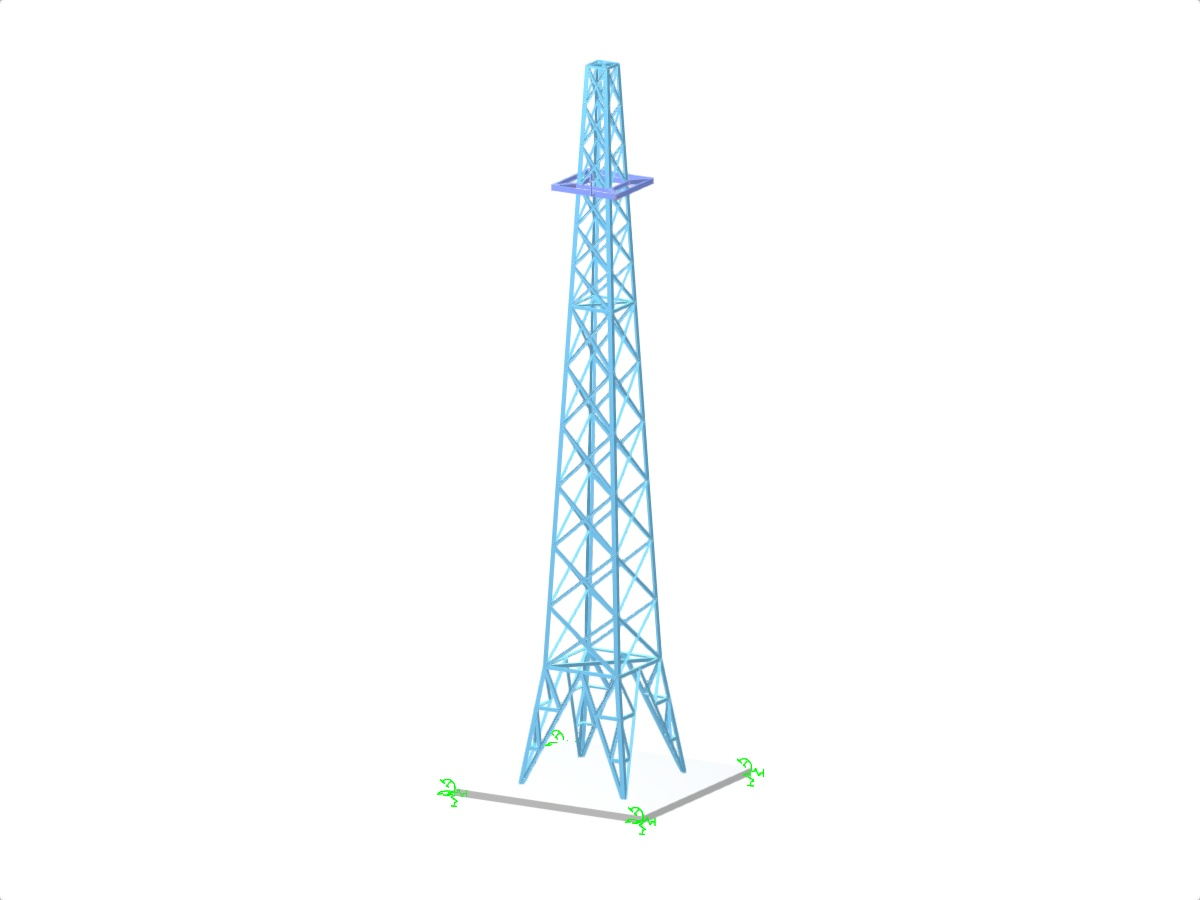
\includegraphics[keepaspectratio]{Figures/Truss_foundation.jpg}}
\caption{Truss\_Foundation}
\end{figure}

    Response spectrum analysis was conducted to evaluate the structural
behavior under dynamic loading conditions. The summary of displacements
obtained from this analysis is presented below.

\begin{longtable}[]{@{}
  >{\raggedright\arraybackslash}p{(\linewidth - 6\tabcolsep) * \real{0.4390}}
  >{\raggedright\arraybackslash}p{(\linewidth - 6\tabcolsep) * \real{0.1220}}
  >{\raggedright\arraybackslash}p{(\linewidth - 6\tabcolsep) * \real{0.1463}}
  >{\raggedright\arraybackslash}p{(\linewidth - 6\tabcolsep) * \real{0.2927}}@{}}
\toprule\noalign{}
\begin{minipage}[b]{\linewidth}\raggedright
Description
\end{minipage} & \begin{minipage}[b]{\linewidth}\raggedright
Value
\end{minipage} & \begin{minipage}[b]{\linewidth}\raggedright
Unit
\end{minipage} & \begin{minipage}[b]{\linewidth}\raggedright
Notes
\end{minipage} \\
\midrule\noalign{}
\endhead
\bottomrule\noalign{}
\endlastfoot
Maximum displacement in X-direction & 653.5 mm & mm & Member No.~313, x:
0.457 m \\
Maximum displacement in Y-direction & 664.1 mm & mm & Member No.~309, x:
0.457 m \\
Maximum displacement in Z-direction & 229.5 mm & mm & FE node No.~177:
(-4.387, 4.387, 30.000 m) \\
Maximum vectorial displacement & 951.7 mm & mm & Member No.~1, x: 0.000
m \\
Maximum rotation about X-axis & 24.6 mrad & mrad & Member No.~365, x:
0.112 m \\
Maximum rotation about Y-axis & 23.7 mrad & mrad & Member No.~150, x:
1.713 m \\
Maximum rotation about Z-axis & 4.5 mrad & mrad & Member No.~119, x:
0.569 m \\
\end{longtable}


\captionsetup{format=plain, labelformat=empty,aboveskip=5pt,belowskip=5pt}
\begin{figure}
\centering
\pandocbounded{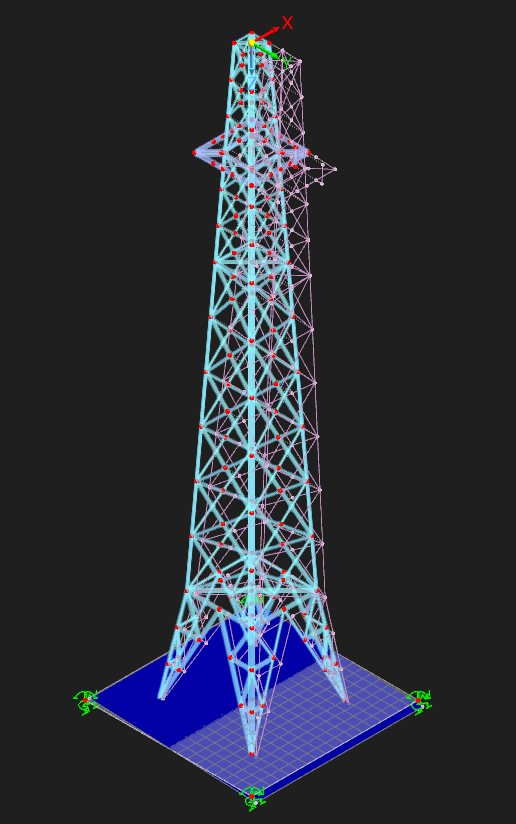
\includegraphics[keepaspectratio]{Figures/m1.png}}
\caption{Modal Shape 1}
\end{figure}

\begin{figure}
\centering
\pandocbounded{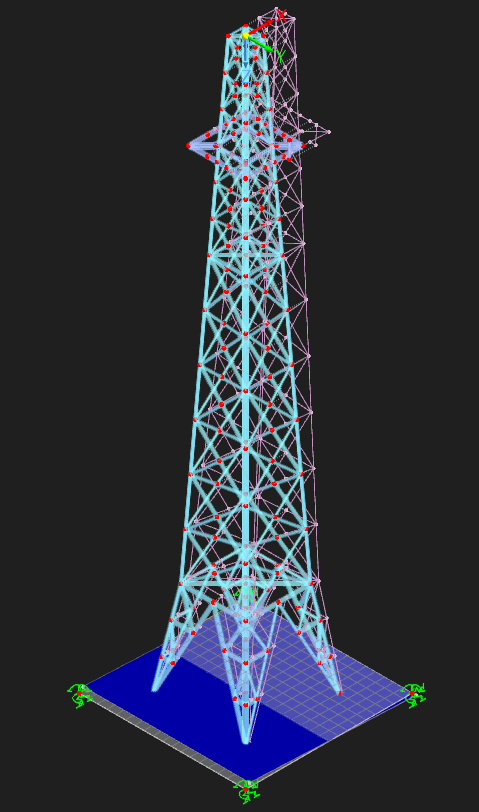
\includegraphics[keepaspectratio]{Figures/m2.png}}
\caption{Modal Shape 2}
\end{figure}

\begin{figure}
\centering
\pandocbounded{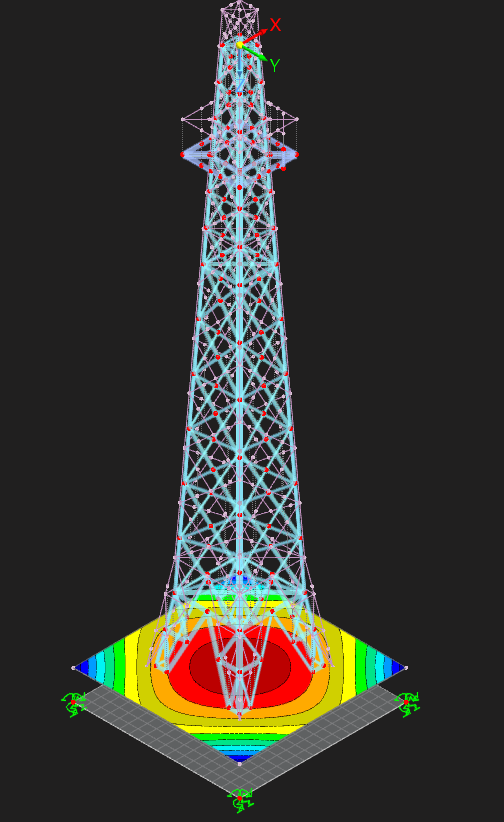
\includegraphics[keepaspectratio]{Figures/m3.png}}
\caption{Modal Shape 3}
\end{figure}


\begin{figure}
\centering
\pandocbounded{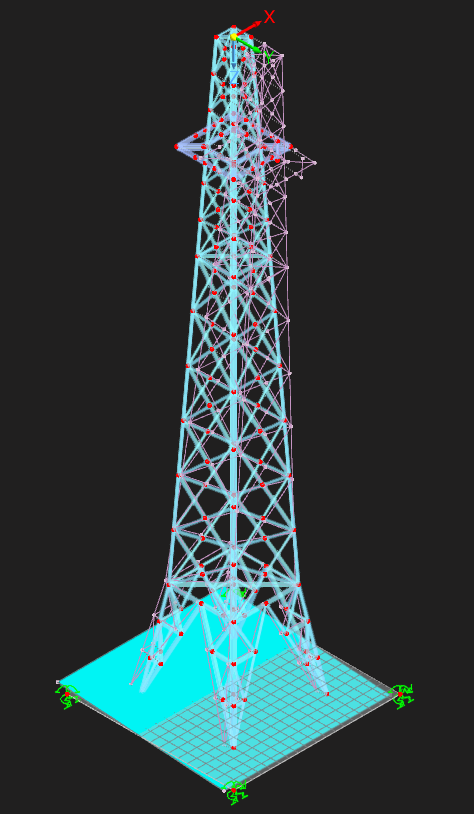
\includegraphics[keepaspectratio]{Figures/m4.png}}
\caption{Modal Shape 4}
\end{figure}

\begin{figure}
\centering
\pandocbounded{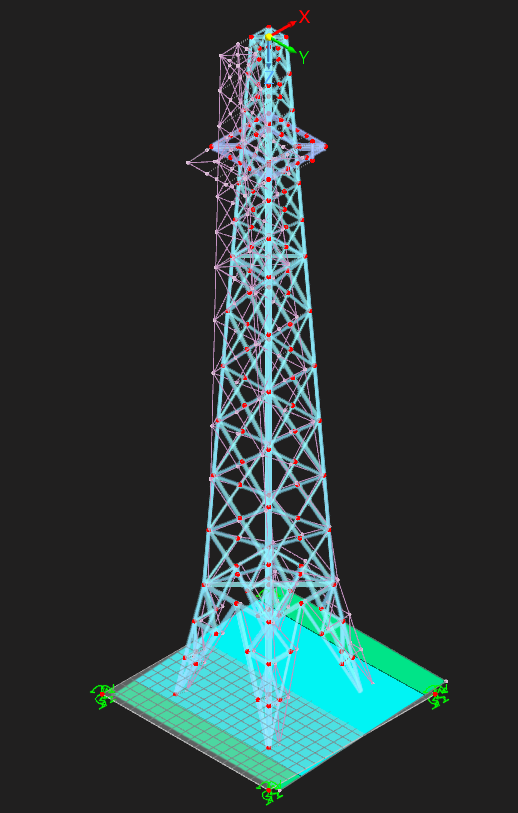
\includegraphics[keepaspectratio]{Figures/m5.png}}
\caption{Modal Shape 5}
\end{figure}
 \captionsetup{format=nocaption,aboveskip=0pt,belowskip=0pt}

    Implementing SSI yields period lengthening that shifts the tower's
natural frequencies to lower values.The distinct modes observed in each
analysis case highlight how foundation and soil properties significantly
alter the load transfer mechanisms from the superstructure to the ground
resulting in non-uniform stress distributions that would not be captured
in a fixed-base analysis. The first two modes are mostly translational
whereas we can see third mode capturing significant vertical
deformations. Mode shapes and modal participation factors become
redistributed, with translational and torsional modes coupling more
strongly, thereby affecting the accuracy of modal combination methods in
RSA. The RSA results with the elastic foundation springs demonstrate a
significant increase in maximum structural displacements compared to the
fixed-support analysis presented earlier.Additionally, since the damping
contribution of soil is neglected, this could further contribute to the
higher observed responses.The higher displacements observed in the
tabulated results reflect the more realistic structural behavior under
seismic loading.These insights underscore the importance of
incorporating SSI in RSA for telecommunication towers to capture
realistic dynamic behavior and avoid under- or over-design based on
rigid support assumptions.

    \subsection{Part B}\label{part-b}

As previously mentioned, mode 2 presents an Effective Modal Mass factor
of 0.45, it was therefore considered the most appropriate to describe
the system in a Single Degree of Freedom simplified system. The mass and
moment of inertia of the SDoF system correspond to the effective modal
mass in the translational x direction and rotational effective mass
about the y-axis of the MDoF model. Both parameters can be extracted
from the finite element model assembled in RFEM. The modal height can be
computed as \(h^*=\frac{\Gamma_{ry}}{\Gamma_t}\). A modal damping ratio
of \(\zeta^*=0.048\) is assumed, therefore \(c^*=2\zeta^*m^*\omega\).
Finally the modal stiffness can be derived as \(k^*= \omega^2 M^*\)

A summary of the properties used in the conversion from MDoF to SDoF is
presented in the following table:

\begin{longtable}[]{@{}ccc@{}}
\toprule\noalign{}
Parameter & Value & Origin \\
\midrule\noalign{}
\endhead
\bottomrule\noalign{}
\endlastfoot
Modal mass & \(1683\ kg\) & RFEM \\
Effective Modal Mass (x) \textgreater{} m & \(3940\ kg\) & RFEM \\
Effective Modal Mass (r-y) \textgreater{} J & \(371117\ kg\cdot m^2\) &
RFEM \\
\(\Gamma_t\) & \(2575\) & RFEM \\
\(\Gamma_{ry}\) & \(24995\) & RFEM \\
\(h^*\) & \(9.705\ m\) & Computed \\
\(c^*\) & \(3724\ kg \cdot rad/s\) & Computed \\
\(k^*\) & \(2092787\ kg \cdot rad^2/s^2\) & Computed \\
\end{longtable}

Taking into account the presence of the soil the SDOF system can
therefore be represented as follows.

\begin{figure}
\centering
\pandocbounded{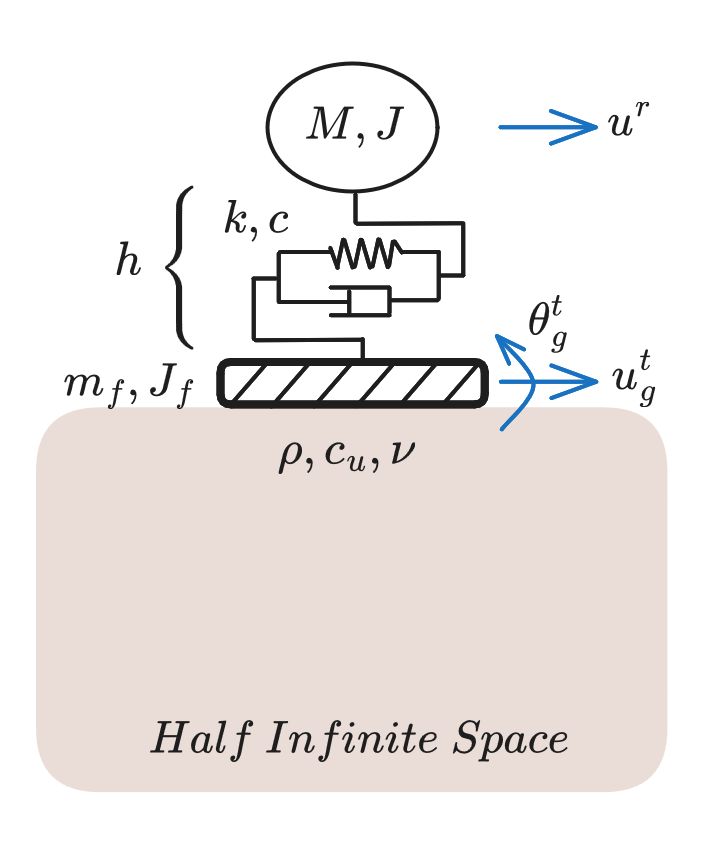
\includegraphics[width=0.45\textwidth]{Figures/SSI_system_diagram.png}}
\caption{SSI\_system}
\end{figure}

Where:

\(u^r(t)\) relative displacement between top mass and foundation

\(u_g^t(t) = u_g(t) + u_g^I(t)\) with: \(u_g^t(t)\) total ground
displacement, \(u_g(t)\) free-field ground displacement, \(u_g^I(t)\)
ground displacement deriving from soil-structure interaction

\(\theta_g^t(t) = \cancel{\theta_g(t)} + \theta_g^I(t)\) with
\(\theta_g^t(t)\) total rocking motion of the ground, \(\theta_g(t)\)
free-field rocking motion (neglected), \(\theta_g^I(t)\) rocking motion
due to soil-structure interaction

The system can then be divided in two subsystems in order to analyze the
interaction between soil and structure.

\begin{figure}
\centering
\pandocbounded{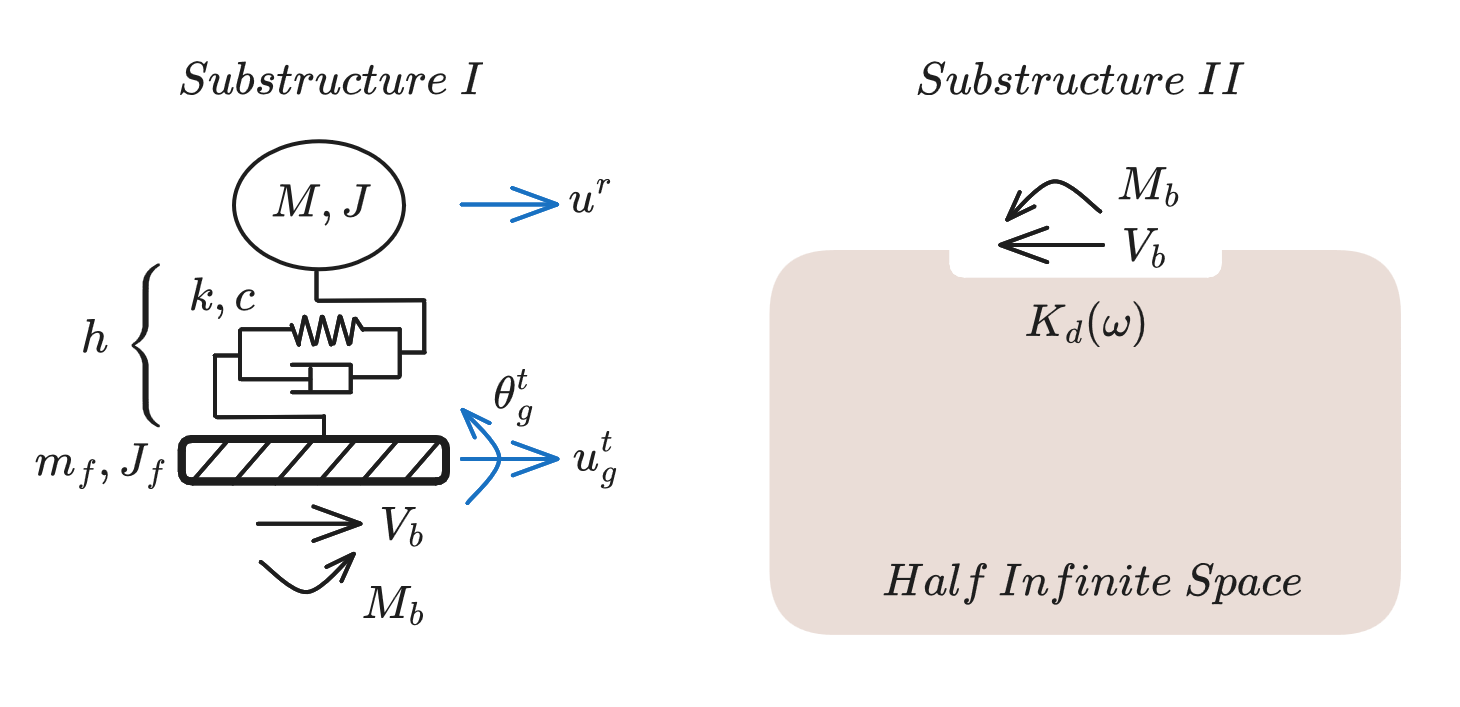
\includegraphics[keepaspectratio]{Figures/SSI_subsystems.png}}
\caption{SSI\_subsystems}
\end{figure}

The translational equilibrium equation for the top mass can be
formulated as:

\(m\ddot{u^r}(t) + c\dot{u^r}(t) + ku^r(t) + m(\ddot{u}_g(t) + \ddot{u}_g^I(t) + h \ddot{\theta}_g^I(t)) = 0\)

The translational equilibrium at soil-structure interface can be
formulated as:

\(m(\ddot{u}_g(t) + \ddot{u}_g^I(t) + \ddot{u^r}(t) + h\ddot{\theta}_g^I(t)) + m_f(\ddot{u}_g(t) + \ddot{u}_g^l(t)) = V_b(t)\)

The rotational equilibrium at the soil-structure interface can be
formulated as:

\(mh(\ddot{u}_g(t) + \ddot{u}_g^l(t) + \ddot{u^r}(t)) + (mh^2 + J + J_f)\ddot{\theta}_g^l(t) = M_b(t)\)

Using a Fourier Transform the system can be converted to the frequency
domain as follows:

\((-\omega^2m + i\omega c + k)\tilde{u^r}(\omega) - \omega^2m\tilde{u}_g^I(\omega) - \omega^2mh\tilde{\theta}_g^I(\omega) = -m\tilde{a_g}(\omega)\)

\(-\omega^2m\tilde{u^r}(\omega) - \omega^2(m + m_f)\tilde{u}_g^I(\omega) - \omega^2mh\tilde{\theta}_g^I(\omega) - \tilde{V}_b(\omega) = -(m + m_f)\tilde{a}_g(\omega)\)

\(-\omega^2mh\tilde{u^r}(\omega) - \omega^2mh\tilde{u}_g^I(\omega) - \omega^2(mh^2 + J + J_f)\tilde{\theta}_g^I(\omega) - \tilde{M}_b(\omega) = -mh\tilde{a}_g(\omega)\)

Where: \(\tilde{a_g} = \tilde{\ddot{u_g}}\)

Moreover
\({\tilde{V}_b(\omega)}^{SS-I} = - {\tilde{V}_b(\omega)}^{SS-II}\) and
\({\tilde{M}_b(\omega)}^{SS-I} = - {\tilde{M}_b(\omega)}^{SS-II}\)

\(\tilde{V}_b(\omega)\) and \(\tilde{M}_b(\omega)\) can therefore be
derived from the soil stiffness matrix as:

\(\tilde{V}_b(\omega) = - \tilde{k}_{xx}(\omega)\tilde{u}_g^I(\omega)-\cancel{\tilde{k}_{x\theta}(\omega)\tilde{\theta}_g^I(\omega)}-i\omega\tilde{c}_{xx}(\omega)\tilde{u}_g^I(\omega)-\cancel{i\omega\tilde{c}_{x\theta}(\omega)\tilde{\theta}_g^I(\omega)}\)

\(\tilde{M}_b(\omega) = - \cancel{\tilde{k}_{\theta x}(\omega)\tilde{u}_g^I(\omega)}-\tilde{k}_{\theta\theta}(\omega)\tilde{\theta}_g^I(\omega)-\cancel{i\omega\tilde{c}_{\theta x}(\omega)\tilde{u}_g^I(\omega)}-i\omega\tilde{c}_{\theta \theta}(\omega)\tilde{\theta}_g^I(\omega)\)

Soil stiffness coefficients were derived following the methodology
presented in Gazetas, G. (1991). Formulas and charts for impedances of
surface and embedded foundations. Journal of Geotechnical Engineering,
117(9), 1363--1381. (see part A). It is worth underlying that
cross-coupling terms (translation-rotation interaction) can be neglected
when dealing with shallow foundations.

After the final substitution, the system can therefore be rewritten in
the following form:

\((-\omega^2m + i\omega c + k)\tilde{u^r}(\omega) - \omega^2m\tilde{u}_g^I(\omega) - \omega^2mh\tilde{\theta}_g^I(\omega) = -m\tilde{a}_g(\omega)\)

\(-\omega^2m\tilde{u^r}(\omega) + (\tilde{k}_{xx}(\omega) + i\omega\tilde{c}_{xx}(\omega) - \omega^2(m + m_f))\tilde{u}_g^I(\omega) - \omega^2mh\tilde{\theta}_g^I(\omega) = -(m + m_f)\tilde{a}_g(\omega)\)

\(-\omega^2mh\tilde{u^r}(\omega) - \omega^2mh\tilde{u}_g^I(\omega) + (\tilde{k}_{\theta\theta}(\omega) + i\omega\tilde{c}_{\theta\theta}(\omega)- \omega^2(mh^2 + J + J_f))\tilde{\theta}_g^I(\omega) = -mh\tilde{a}_g(\omega)\)

The algebraic system of equations can be solved for the three unknowns:
\(\tilde{u^r}(\omega)\), \(\tilde{u}_g^I(\omega)\),
\(\tilde{\theta}_g^I(\omega)\)

By adopting an analogous approach the system without soil structure
interaction could be described by the following equations:

Equation of motion:
\(m\ddot{u^r}(t) + c\dot{u^r}(t) + ku^r(t) =  -ma_{g} - \cancel{mh\theta_{g}}\)

Equation of motion in frequency domain
\((-\omega^2m + i\omega c + k)\tilde{u^r}(\omega) = -m\tilde{a}_{g}(\omega)\)

    \begin{tcolorbox}[breakable, size=fbox, boxrule=1pt, pad at break*=1mm,colback=cellbackground, colframe=cellborder]
\prompt{In}{incolor}{5}{\boxspacing}
\begin{Verbatim}[commandchars=\\\{\}]
\PY{c+c1}{\PYZsh{} SDOF Model }
\PY{n}{m\PYZus{}modal} \PY{o}{=} \PY{l+m+mi}{1683}     \PY{c+c1}{\PYZsh{}[kg] modal mass}
\PY{n}{M\PYZus{}x} \PY{o}{=} \PY{l+m+mi}{3940}         \PY{c+c1}{\PYZsh{}[kg] effective translational modal mass in the x direction}
\PY{n}{J\PYZus{}y} \PY{o}{=} \PY{l+m+mi}{371117}       \PY{c+c1}{\PYZsh{}[kg*m\PYZca{}2] effective rotational modal mass about the y\PYZhy{}axis (moment of inertia)}
\PY{n}{gamma\PYZus{}t} \PY{o}{=} \PY{l+m+mf}{2575.4}   \PY{c+c1}{\PYZsh{}[\PYZhy{}] translational participation factor in the x direction}
\PY{n}{gamma\PYZus{}ry} \PY{o}{=} \PY{l+m+mf}{24995.1} \PY{c+c1}{\PYZsh{}[\PYZhy{}] rotation participation factor about the y\PYZhy{}axis }
\PY{n}{zeta\PYZus{}star} \PY{o}{=} \PY{l+m+mf}{0.048}  \PY{c+c1}{\PYZsh{}[\PYZhy{}] modal damping ratio (mode 2, arbitrarily assumed)}
\PY{n}{omega\PYZus{}s} \PY{o}{=} \PY{l+m+mf}{23.044}   \PY{c+c1}{\PYZsh{}[rad/s] natural frequency of the SDoF model (mode 2)}

\PY{n}{h\PYZus{}star} \PY{o}{=} \PY{n}{gamma\PYZus{}ry}\PY{o}{/}\PY{n}{gamma\PYZus{}t}
\PY{n}{c\PYZus{}star} \PY{o}{=} \PY{l+m+mi}{2}\PY{o}{*}\PY{n}{zeta\PYZus{}star}\PY{o}{*}\PY{n}{m\PYZus{}modal}\PY{o}{*}\PY{n}{omega\PYZus{}s}
\PY{n}{k\PYZus{}star} \PY{o}{=} \PY{n}{omega\PYZus{}s}\PY{o}{*}\PY{o}{*}\PY{l+m+mi}{2}\PY{o}{*}\PY{n}{M\PYZus{}x}

\PY{n}{rho\PYZus{}f} \PY{o}{=} \PY{l+m+mi}{2400} \PY{c+c1}{\PYZsh{}[kg/m\PYZca{}3] Density of concrete (arbitrarily chosen)}
\PY{n}{m\PYZus{}f} \PY{o}{=} \PY{n}{rho\PYZus{}f}\PY{o}{*}\PY{n}{side\PYZus{}x}\PY{o}{*}\PY{n}{side\PYZus{}y}\PY{o}{*}\PY{n}{depth} \PY{c+c1}{\PYZsh{}[kg] Mass of foundation}
\PY{n}{J\PYZus{}y\PYZus{}f} \PY{o}{=} \PY{n}{m\PYZus{}f}\PY{o}{*}\PY{p}{(}\PY{n}{side\PYZus{}x}\PY{o}{*}\PY{o}{*}\PY{l+m+mi}{2}\PY{o}{+}\PY{n}{depth}\PY{o}{*}\PY{o}{*}\PY{l+m+mi}{2}\PY{p}{)}\PY{o}{/}\PY{l+m+mi}{12} \PY{c+c1}{\PYZsh{}[kg*m\PYZca{}2] Moment of Inertia of foundation about the y\PYZhy{}axis}

\PY{n+nb}{print}\PY{p}{(}\PY{l+s+s2}{\PYZdq{}}\PY{l+s+s2}{Parameter Recap:}\PY{l+s+s2}{\PYZdq{}}\PY{p}{)}
\PY{n+nb}{print}\PY{p}{(}\PY{l+s+sa}{f}\PY{l+s+s2}{\PYZdq{}}\PY{l+s+s2}{h\PYZus{}star: }\PY{l+s+si}{\PYZob{}}\PY{n}{h\PYZus{}star}\PY{l+s+si}{:}\PY{l+s+s2}{.3f}\PY{l+s+si}{\PYZcb{}}\PY{l+s+s2}{ m}\PY{l+s+s2}{\PYZdq{}}\PY{p}{)}
\PY{n+nb}{print}\PY{p}{(}\PY{l+s+sa}{f}\PY{l+s+s2}{\PYZdq{}}\PY{l+s+s2}{c\PYZus{}star: }\PY{l+s+si}{\PYZob{}}\PY{n}{c\PYZus{}star}\PY{l+s+si}{:}\PY{l+s+s2}{.3f}\PY{l+s+si}{\PYZcb{}}\PY{l+s+s2}{ kg*rad/s}\PY{l+s+s2}{\PYZdq{}}\PY{p}{)}
\PY{n+nb}{print}\PY{p}{(}\PY{l+s+sa}{f}\PY{l+s+s2}{\PYZdq{}}\PY{l+s+s2}{k\PYZus{}star: }\PY{l+s+si}{\PYZob{}}\PY{n}{k\PYZus{}star}\PY{l+s+si}{:}\PY{l+s+s2}{.3f}\PY{l+s+si}{\PYZcb{}}\PY{l+s+s2}{ kg*rad\PYZca{}2/s\PYZca{}2}\PY{l+s+s2}{\PYZdq{}}\PY{p}{)}

\PY{n}{omega\PYZus{}table\PYZus{}max} \PY{o}{=} \PY{l+m+mi}{2}\PY{o}{*}\PY{n}{v\PYZus{}s}\PY{o}{/}\PY{n}{B}
\PY{n}{omega\PYZus{}domain} \PY{o}{=} \PY{n}{np}\PY{o}{.}\PY{n}{linspace}\PY{p}{(}\PY{l+m+mf}{0.001}\PY{p}{,} \PY{n}{omega\PYZus{}table\PYZus{}max}\PY{p}{,}\PY{l+m+mi}{10000}\PY{p}{)} \PY{c+c1}{\PYZsh{}Based on curves applicability (domain from tables)}

\PY{c+c1}{\PYZsh{} Fitting of curves in tables}
\PY{c+c1}{\PYZsh{}\PYZsh{} Only c\PYZus{}ry}
\PY{n}{points} \PY{o}{=} \PY{p}{[}\PY{p}{[}\PY{l+m+mi}{0}\PY{p}{,} \PY{l+m+mf}{0.25}\PY{p}{,} \PY{l+m+mf}{0.5}\PY{p}{,} \PY{l+m+mf}{0.65}\PY{p}{,} \PY{l+m+mi}{1}\PY{p}{,} \PY{l+m+mf}{1.5}\PY{p}{,} \PY{l+m+mi}{2}\PY{p}{]}\PY{p}{,}\PY{p}{[}\PY{l+m+mi}{0}\PY{p}{,} \PY{l+m+mf}{0.05}\PY{p}{,} \PY{l+m+mf}{0.125}\PY{p}{,} \PY{l+m+mf}{0.2}\PY{p}{,} \PY{l+m+mf}{0.3}\PY{p}{,} \PY{l+m+mf}{0.45}\PY{p}{,} \PY{l+m+mf}{0.55}\PY{p}{]}\PY{p}{]}
\PY{n}{c\PYZus{}ry\PYZus{}curve} \PY{o}{=} \PY{n}{np}\PY{o}{.}\PY{n}{poly1d}\PY{p}{(}\PY{n}{np}\PY{o}{.}\PY{n}{polyfit}\PY{p}{(}\PY{n}{points}\PY{p}{[}\PY{l+m+mi}{0}\PY{p}{]}\PY{p}{,} \PY{n}{points}\PY{p}{[}\PY{l+m+mi}{1}\PY{p}{]}\PY{p}{,} \PY{l+m+mi}{5}\PY{p}{)}\PY{p}{)}

\PY{c+c1}{\PYZsh{} Polynomial graph as sanity check}
\PY{c+c1}{\PYZsh{} plt.plot(omega\PYZus{}domain, c\PYZus{}ry\PYZus{}curve(omega\PYZus{}domain*B/v\PYZus{}s))}
\PY{c+c1}{\PYZsh{} plt.show()}

\PY{n}{frf\PYZus{}ur\PYZus{}tilde} \PY{o}{=} \PY{p}{[}\PY{p}{]}
\PY{n}{frf\PYZus{}ug\PYZus{}tilde} \PY{o}{=} \PY{p}{[}\PY{p}{]}
\PY{n}{frf\PYZus{}thetag\PYZus{}tilde} \PY{o}{=} \PY{p}{[}\PY{p}{]}

\PY{k}{for} \PY{n}{counter}\PY{p}{,}\PY{n}{omega} \PY{o+ow}{in} \PY{n+nb}{enumerate}\PY{p}{(}\PY{n}{omega\PYZus{}domain}\PY{p}{)}\PY{p}{:}

    \PY{c+c1}{\PYZsh{} Frequency Dependent Coefficients for Dynamic Stiffness and Damping of Soil }
    \PY{c+c1}{\PYZsh{} (same as previous code\PYZhy{}cell but repeated inside the loop only for relevant directions of motion, necessary to account for frequency dependency)}
    \PY{n}{a\PYZus{}0} \PY{o}{=} \PY{n}{omega}\PY{o}{*}\PY{n}{B}\PY{o}{/}\PY{n}{v\PYZus{}s}

    \PY{n}{K\PYZus{}y\PYZus{}static} \PY{o}{=} \PY{p}{(}\PY{l+m+mi}{2}\PY{o}{*}\PY{n}{G}\PY{o}{*}\PY{n}{L}\PY{o}{/}\PY{p}{(}\PY{l+m+mi}{2}\PY{o}{\PYZhy{}}\PY{n}{nu}\PY{p}{)}\PY{p}{)}\PY{o}{*}\PY{p}{(}\PY{l+m+mi}{2}\PY{o}{+}\PY{l+m+mf}{2.50}\PY{o}{*}\PY{n}{chi}\PY{o}{*}\PY{o}{*}\PY{l+m+mf}{0.85}\PY{p}{)} \PY{c+c1}{\PYZsh{}y coefficient is required to compute K\PYZus{}x\PYZus{}static}
    \PY{n}{K\PYZus{}x\PYZus{}static} \PY{o}{=} \PY{n}{K\PYZus{}y\PYZus{}static} \PY{o}{\PYZhy{}} \PY{p}{(}\PY{l+m+mf}{0.2}\PY{o}{/}\PY{p}{(}\PY{l+m+mf}{0.75}\PY{o}{\PYZhy{}}\PY{n}{nu}\PY{p}{)}\PY{p}{)}\PY{o}{*}\PY{n}{G}\PY{o}{*}\PY{n}{L}\PY{o}{*}\PY{p}{(}\PY{l+m+mi}{1}\PY{o}{\PYZhy{}}\PY{p}{(}\PY{n}{B}\PY{o}{/}\PY{n}{L}\PY{p}{)}\PY{p}{)}
    \PY{n}{K\PYZus{}x\PYZus{}dyn} \PY{o}{=} \PY{n}{K\PYZus{}x\PYZus{}static}\PY{o}{*}\PY{l+m+mi}{1} \PY{c+c1}{\PYZsh{}Formula from table}
    \PY{n}{K\PYZus{}ry\PYZus{}static} \PY{o}{=} \PY{p}{(}\PY{l+m+mi}{3}\PY{o}{*}\PY{n}{G}\PY{o}{/}\PY{p}{(}\PY{l+m+mi}{1}\PY{o}{\PYZhy{}}\PY{n}{nu}\PY{p}{)}\PY{p}{)}\PY{o}{*}\PY{n}{I\PYZus{}by}\PY{o}{*}\PY{o}{*}\PY{l+m+mf}{0.75}\PY{o}{*}\PY{p}{(}\PY{n}{L}\PY{o}{/}\PY{n}{B}\PY{p}{)}\PY{o}{*}\PY{o}{*}\PY{l+m+mf}{0.15}
    \PY{n}{K\PYZus{}ry\PYZus{}dyn} \PY{o}{=} \PY{p}{(}\PY{l+m+mi}{1}\PY{o}{\PYZhy{}}\PY{l+m+mf}{0.26}\PY{o}{*}\PY{n}{a\PYZus{}0}\PY{p}{)} \PY{o}{*} \PY{n}{K\PYZus{}ry\PYZus{}static}
    
    \PY{n}{C\PYZus{}x} \PY{o}{=} \PY{n}{rho}\PY{o}{*}\PY{n}{v\PYZus{}s}\PY{o}{*}\PY{n}{A\PYZus{}b} 
    \PY{n}{C\PYZus{}x\PYZus{}tot} \PY{o}{=} \PY{n}{C\PYZus{}x} \PY{o}{+} \PY{l+m+mi}{2}\PY{o}{*}\PY{n}{K\PYZus{}x\PYZus{}dyn}\PY{o}{*}\PY{n}{beta}\PY{o}{/}\PY{n}{omega} 
    \PY{n}{C\PYZus{}ry} \PY{o}{=} \PY{n}{rho}\PY{o}{*}\PY{n}{v\PYZus{}la}\PY{o}{*}\PY{n}{I\PYZus{}by}\PY{o}{*}\PY{n}{c\PYZus{}ry\PYZus{}curve}\PY{p}{(}\PY{n}{a\PYZus{}0}\PY{p}{)}
    \PY{n}{C\PYZus{}ry\PYZus{}tot} \PY{o}{=} \PY{n}{C\PYZus{}ry} \PY{o}{+} \PY{l+m+mi}{2}\PY{o}{*}\PY{n}{K\PYZus{}ry\PYZus{}dyn}\PY{o}{*}\PY{n}{beta}\PY{o}{/}\PY{n}{omega} 

    \PY{c+c1}{\PYZsh{} Acceleration}
    \PY{n}{a\PYZus{}g\PYZus{}tilde} \PY{o}{=} \PY{l+m+mi}{1} \PY{c+c1}{\PYZsh{}[(m/s\PYZca{}2)/Hz] Acceleration in the frequency domain (taken as unitary for FRF computation) }

    \PY{n}{K\PYZus{}tilde\PYZus{}system} \PY{o}{=} \PY{n}{np}\PY{o}{.}\PY{n}{zeros}\PY{p}{(}\PY{p}{(}\PY{l+m+mi}{3}\PY{p}{,}\PY{l+m+mi}{3}\PY{p}{)}\PY{p}{,} \PY{n}{dtype}\PY{o}{=}\PY{n+nb}{complex}\PY{p}{)}
    \PY{n}{K\PYZus{}tilde\PYZus{}system}\PY{p}{[}\PY{l+m+mi}{0}\PY{p}{,} \PY{l+m+mi}{0}\PY{p}{]} \PY{o}{=} \PY{o}{\PYZhy{}}\PY{n}{omega}\PY{o}{*}\PY{o}{*}\PY{l+m+mi}{2}\PY{o}{*}\PY{n}{M\PYZus{}x} \PY{o}{+} \PY{l+m+mi}{1}\PY{n}{j}\PY{o}{*}\PY{n}{omega}\PY{o}{*}\PY{n}{c\PYZus{}star} \PY{o}{+} \PY{n}{k\PYZus{}star}
    \PY{n}{K\PYZus{}tilde\PYZus{}system}\PY{p}{[}\PY{l+m+mi}{1}\PY{p}{,} \PY{l+m+mi}{1}\PY{p}{]} \PY{o}{=} \PY{n}{K\PYZus{}x\PYZus{}dyn} \PY{o}{+} \PY{l+m+mi}{1}\PY{n}{j}\PY{o}{*}\PY{n}{omega}\PY{o}{*}\PY{n}{C\PYZus{}x\PYZus{}tot} \PY{o}{\PYZhy{}} \PY{n}{omega}\PY{o}{*}\PY{o}{*}\PY{l+m+mi}{2}\PY{o}{*}\PY{p}{(}\PY{n}{M\PYZus{}x}\PY{o}{+}\PY{n}{m\PYZus{}f}\PY{p}{)}
    \PY{n}{K\PYZus{}tilde\PYZus{}system}\PY{p}{[}\PY{l+m+mi}{2}\PY{p}{,} \PY{l+m+mi}{2}\PY{p}{]} \PY{o}{=} \PY{n}{K\PYZus{}ry\PYZus{}dyn} \PY{o}{+} \PY{l+m+mi}{1}\PY{n}{j}\PY{o}{*}\PY{n}{omega}\PY{o}{*}\PY{n}{C\PYZus{}ry\PYZus{}tot} \PY{o}{\PYZhy{}} \PY{n}{omega}\PY{o}{*}\PY{o}{*}\PY{l+m+mi}{2}\PY{o}{*}\PY{p}{(}\PY{n}{M\PYZus{}x}\PY{o}{*}\PY{n}{h\PYZus{}star}\PY{o}{*}\PY{o}{*}\PY{l+m+mi}{2}\PY{o}{+}\PY{n}{J\PYZus{}y}\PY{o}{+}\PY{n}{J\PYZus{}y\PYZus{}f}\PY{p}{)}
    \PY{n}{K\PYZus{}tilde\PYZus{}system}\PY{p}{[}\PY{l+m+mi}{0}\PY{p}{,} \PY{l+m+mi}{1}\PY{p}{]} \PY{o}{=} \PY{n}{K\PYZus{}tilde\PYZus{}system}\PY{p}{[}\PY{l+m+mi}{1}\PY{p}{,} \PY{l+m+mi}{0}\PY{p}{]} \PY{o}{=} \PY{o}{\PYZhy{}}\PY{n}{omega}\PY{o}{*}\PY{o}{*}\PY{l+m+mi}{2}\PY{o}{*}\PY{n}{M\PYZus{}x}
    \PY{n}{K\PYZus{}tilde\PYZus{}system}\PY{p}{[}\PY{l+m+mi}{0}\PY{p}{,} \PY{l+m+mi}{2}\PY{p}{]} \PY{o}{=} \PY{n}{K\PYZus{}tilde\PYZus{}system}\PY{p}{[}\PY{l+m+mi}{2}\PY{p}{,} \PY{l+m+mi}{0}\PY{p}{]} \PY{o}{=} \PY{o}{\PYZhy{}}\PY{n}{omega}\PY{o}{*}\PY{o}{*}\PY{l+m+mi}{2}\PY{o}{*}\PY{n}{M\PYZus{}x}\PY{o}{*}\PY{n}{h\PYZus{}star}
    \PY{n}{K\PYZus{}tilde\PYZus{}system}\PY{p}{[}\PY{l+m+mi}{1}\PY{p}{,} \PY{l+m+mi}{2}\PY{p}{]} \PY{o}{=} \PY{n}{K\PYZus{}tilde\PYZus{}system}\PY{p}{[}\PY{l+m+mi}{2}\PY{p}{,} \PY{l+m+mi}{1}\PY{p}{]} \PY{o}{=} \PY{o}{\PYZhy{}} \PY{n}{omega}\PY{o}{*}\PY{o}{*}\PY{l+m+mi}{2}\PY{o}{*}\PY{n}{M\PYZus{}x}\PY{o}{*}\PY{n}{h\PYZus{}star}

    \PY{n}{F\PYZus{}tilde} \PY{o}{=} \PY{n}{np}\PY{o}{.}\PY{n}{array}\PY{p}{(}\PY{p}{[}\PY{o}{\PYZhy{}}\PY{n}{M\PYZus{}x}\PY{o}{*}\PY{n}{a\PYZus{}g\PYZus{}tilde}\PY{p}{,} \PY{o}{\PYZhy{}}\PY{p}{(}\PY{n}{M\PYZus{}x}\PY{o}{+}\PY{n}{m\PYZus{}f}\PY{p}{)}\PY{o}{*}\PY{n}{a\PYZus{}g\PYZus{}tilde}\PY{p}{,} \PY{o}{\PYZhy{}}\PY{n}{M\PYZus{}x}\PY{o}{*}\PY{n}{h\PYZus{}star}\PY{o}{*}\PY{n}{a\PYZus{}g\PYZus{}tilde}\PY{p}{]}\PY{p}{)}
    
    \PY{n}{u\PYZus{}r\PYZus{}tilde\PYZus{}omega} \PY{p}{,} \PY{n}{ug\PYZus{}tilde\PYZus{}omega} \PY{p}{,} \PY{n}{u\PYZus{}thetag\PYZus{}tilde\PYZus{}omega}  \PY{o}{=} \PY{n}{np}\PY{o}{.}\PY{n}{linalg}\PY{o}{.}\PY{n}{solve}\PY{p}{(}\PY{n}{K\PYZus{}tilde\PYZus{}system}\PY{p}{,} \PY{n}{F\PYZus{}tilde}\PY{p}{)}
    \PY{n}{frf\PYZus{}ur\PYZus{}tilde}\PY{o}{.}\PY{n}{append}\PY{p}{(}\PY{n}{u\PYZus{}r\PYZus{}tilde\PYZus{}omega}\PY{p}{)}
    \PY{n}{frf\PYZus{}ug\PYZus{}tilde}\PY{o}{.}\PY{n}{append}\PY{p}{(}\PY{n}{ug\PYZus{}tilde\PYZus{}omega}\PY{p}{)}
    \PY{n}{frf\PYZus{}thetag\PYZus{}tilde}\PY{o}{.}\PY{n}{append}\PY{p}{(}\PY{n}{u\PYZus{}thetag\PYZus{}tilde\PYZus{}omega}\PY{p}{)}


\PY{c+c1}{\PYZsh{} No\PYZhy{}interaction SDOF response}

\PY{n}{frf\PYZus{}ur\PYZus{}tilde\PYZus{}no\PYZus{}SSI} \PY{o}{=} \PY{p}{[}\PY{o}{\PYZhy{}}\PY{n}{M\PYZus{}x}\PY{o}{*}\PY{n}{a\PYZus{}g\PYZus{}tilde}\PY{o}{/}\PY{p}{(}\PY{o}{\PYZhy{}}\PY{n}{omega}\PY{o}{*}\PY{o}{*}\PY{l+m+mi}{2}\PY{o}{*}\PY{n}{M\PYZus{}x}\PY{o}{+}\PY{l+m+mi}{1}\PY{n}{j}\PY{o}{*}\PY{n}{c\PYZus{}star}\PY{o}{*}\PY{n}{omega}\PY{o}{+}\PY{n}{k\PYZus{}star}\PY{p}{)} \PY{k}{for} \PY{n}{omega} \PY{o+ow}{in} \PY{n}{omega\PYZus{}domain}\PY{p}{]}

\PY{n}{plt}\PY{o}{.}\PY{n}{semilogy}\PY{p}{(}\PY{n}{omega\PYZus{}domain}\PY{p}{,} \PY{n}{np}\PY{o}{.}\PY{n}{abs}\PY{p}{(}\PY{n}{frf\PYZus{}ur\PYZus{}tilde\PYZus{}no\PYZus{}SSI}\PY{p}{)}\PY{p}{,} \PY{n}{label}\PY{o}{=}\PY{l+s+sa}{r}\PY{l+s+s2}{\PYZdq{}}\PY{l+s+s2}{\PYZdl{}Structure}\PY{l+s+s2}{\PYZbs{}}\PY{l+s+s2}{ (excluding}\PY{l+s+s2}{\PYZbs{}}\PY{l+s+s2}{ SSI)\PYZdl{}}\PY{l+s+s2}{\PYZdq{}}\PY{p}{)}
\PY{n}{plt}\PY{o}{.}\PY{n}{semilogy}\PY{p}{(}\PY{n}{omega\PYZus{}domain}\PY{p}{,} \PY{n}{np}\PY{o}{.}\PY{n}{abs}\PY{p}{(}\PY{n}{frf\PYZus{}ur\PYZus{}tilde}\PY{p}{)}\PY{p}{,} \PY{n}{label}\PY{o}{=}\PY{l+s+sa}{r}\PY{l+s+s2}{\PYZdq{}}\PY{l+s+s2}{\PYZdl{}Structure}\PY{l+s+s2}{\PYZbs{}}\PY{l+s+s2}{ (including}\PY{l+s+s2}{\PYZbs{}}\PY{l+s+s2}{ SSI)\PYZdl{}}\PY{l+s+s2}{\PYZdq{}}\PY{p}{)}
\PY{n}{plt}\PY{o}{.}\PY{n}{semilogy}\PY{p}{(}\PY{n}{omega\PYZus{}domain}\PY{p}{,} \PY{n}{np}\PY{o}{.}\PY{n}{abs}\PY{p}{(}\PY{n}{frf\PYZus{}ug\PYZus{}tilde}\PY{p}{)}\PY{p}{,} \PY{n}{label}\PY{o}{=}\PY{l+s+sa}{r}\PY{l+s+s2}{\PYZdq{}}\PY{l+s+s2}{\PYZdl{}Foundation}\PY{l+s+s2}{\PYZbs{}}\PY{l+s+s2}{ Translation\PYZdl{}}\PY{l+s+s2}{\PYZdq{}}\PY{p}{)}
\PY{n}{plt}\PY{o}{.}\PY{n}{semilogy}\PY{p}{(}\PY{n}{omega\PYZus{}domain}\PY{p}{,} \PY{n}{np}\PY{o}{.}\PY{n}{abs}\PY{p}{(}\PY{n}{frf\PYZus{}thetag\PYZus{}tilde}\PY{p}{)}\PY{p}{,} \PY{n}{label}\PY{o}{=}\PY{l+s+sa}{r}\PY{l+s+s2}{\PYZdq{}}\PY{l+s+s2}{\PYZdl{}Foundation}\PY{l+s+s2}{\PYZbs{}}\PY{l+s+s2}{ Rotation\PYZdl{}}\PY{l+s+s2}{\PYZdq{}}\PY{p}{)}
\PY{n}{plt}\PY{o}{.}\PY{n}{title}\PY{p}{(}\PY{l+s+s2}{\PYZdq{}}\PY{l+s+s2}{FRF Comparison between free\PYZhy{}SDoF system and SSI}\PY{l+s+s2}{\PYZdq{}}\PY{p}{)}
\PY{n}{plt}\PY{o}{.}\PY{n}{xlabel}\PY{p}{(}\PY{l+s+sa}{r}\PY{l+s+s2}{\PYZdq{}}\PY{l+s+s2}{\PYZdl{}Frequency}\PY{l+s+s2}{\PYZbs{}}\PY{l+s+s2}{ [rad/s]\PYZdl{}}\PY{l+s+s2}{\PYZdq{}}\PY{p}{)}
\PY{n}{plt}\PY{o}{.}\PY{n}{ylabel}\PY{p}{(}\PY{l+s+sa}{r}\PY{l+s+s2}{\PYZdq{}}\PY{l+s+s2}{\PYZdl{}Motion}\PY{l+s+s2}{\PYZbs{}}\PY{l+s+s2}{ [m/Hz]\PYZdl{}}\PY{l+s+s2}{\PYZdq{}}\PY{p}{)}
\PY{n}{plt}\PY{o}{.}\PY{n}{grid}\PY{p}{(}\PY{p}{)}
\PY{c+c1}{\PYZsh{} plt.xlim(0, 10)}
\PY{n}{plt}\PY{o}{.}\PY{n}{legend}\PY{p}{(}\PY{p}{)}
\end{Verbatim}
\end{tcolorbox}

    \begin{Verbatim}[commandchars=\\\{\}]
Parameter Recap:
h\_star: 9.705 m
c\_star: 3723.173 kg*rad/s
k\_star: 2092242.188 kg*rad\^{}2/s\^{}2
    \end{Verbatim}

            \begin{tcolorbox}[breakable, size=fbox, boxrule=.5pt, pad at break*=1mm, opacityfill=0]
\prompt{Out}{outcolor}{5}{\boxspacing}
\begin{Verbatim}[commandchars=\\\{\}]
<matplotlib.legend.Legend at 0x25d5d88c440>
\end{Verbatim}
\end{tcolorbox}
        
    \begin{center}
    \adjustimage{max size={0.9\linewidth}{0.9\paperheight}}{output_17_2.png}
    \end{center}
    { \hspace*{\fill} \\}
    
    It is apparent how the introduction of the SSI has a significant impact
on the dynamic response of the system. This is not only due to the soil
behavior but also to the introduction of the foundation mass and the
related degrees of freedom. The FRF of the structure inclusive of the
interaction model shows a shifted and milder peak in the natural
frequency corresponding to the vibration of the top mass. From the
standpoint of the physical accuracy of the model, an important addition
compared to the SDoF system without SSI is the energy dissipation due to
soil material damping and radiation damping. Moreover a second peak
appears in the structure response. Such peak is located at approximately
3 Hz and corresponds to the natural frequency of the rotational degree
of freedom of the foundation.


    % Add a bibliography block to the postdoc
    
    
    
\end{document}
